\documentclass[10pt,a4paper]{article}

\usepackage[utf8]{inputenc}
\usepackage[T1]{fontenc}
\usepackage{lmodern}
\usepackage[top=2.0cm,bottom=2.0cm,left=2.0cm,right=2.0cm]{geometry}
\usepackage{amsmath,amssymb,amsfonts}
\usepackage{booktabs}
\usepackage{multirow}
\usepackage{array}
\usepackage{graphicx}
\graphicspath{{../}{./}{../figures/}{figures/}}
\usepackage{subcaption}
\usepackage{float}
\usepackage{xcolor}
\usepackage{hyperref}
\usepackage{enumitem}
\usepackage{caption}

% Typography and spacing matching clean peer reports
\setlength{\parindent}{0pt}
\setlength{\parskip}{4.5pt plus 1pt minus 1pt}
\setlength{\intextsep}{10pt plus 2pt minus 2pt}
\setlength{\textfloatsep}{10pt plus 2pt minus 2pt}
\setlength{\floatsep}{8pt plus 2pt minus 2pt}
\renewcommand{\arraystretch}{1.05}
\captionsetup{font=small,labelfont=bf,aboveskip=5pt,belowskip=3pt}

\hypersetup{
    colorlinks=true,
    linkcolor=blue!70!black,
    citecolor=blue!70!black,
    urlcolor=blue!70!black
}

\title{\Large \textbf{Qubit Evolution: Predicting Quantum Dynamics with Deep Learning}\vspace{-0.2cm}}
\author{
    \textsc{Ernesto Gligora} \qquad \textsc{Riccardo Lavorato} \\[2pt]
    \small \textit{Artificial Intelligence and Computer Science / University of Calabria}
}
\date{\vspace{-0.3cm}\small Academic Year 2025/2026\vspace{-0.2cm}}

\begin{document}

\maketitle

\begin{abstract}
\noindent
Simulating interacting quantum many-body systems is computationally expensive on classical computers: the state space grows exponentially as $2^N$, and quantum entanglement creates complex spatial and temporal correlations. In this project, we use deep learning sequence models to learn and forecast qubit dynamics from short observation windows. We study the $N = 10$ qubit PXP Rydberg-blockade Hamiltonian across $D = 55$ continuous physical observables ($10$ local magnetizations and $45$ pairwise correlations) over $400$ simulated trajectories. Following a rigorous incremental workflow, we first evaluate a preliminary pilot study on $20$ trajectories and test dimensionality reduction via an Autoencoder ($55 \to 16 \to 55$), showing that operating directly on native observables avoids an irreducible reconstruction bottleneck ($3.62 \times 10^{-4}$). We then implement and benchmark four sequence architectures across Recurrent (M1, M2) and Transformer (M3, M4) families, trained under a unified 25-epoch hybrid curriculum (Teacher Forcing $\to$ Masked Modeling $\to$ Scheduled Sampling). Across our 24-model factorial benchmark, the compact one-shot Transformer \textbf{M3 (HP3)} ($196{,}632$ parameters) achieves the best overall performance ($\text{Val MSE} = 1.21 \times 10^{-4}$, $\text{Test MSE} = 1.21 \times 10^{-4}$, $\text{Test MAE} = 0.00785$), improving by $25\%$ over the best RNN \textbf{M1 (HP1)} ($\text{Test MSE} = 1.61 \times 10^{-4}$) with zero violations of quantum density-matrix positivity ($P(s_i, s_j) \ge 0$, $P_{\min} = 0.1632$). Finally, we resolve all three project challenges: (1) an aligned window ablation proves that $T_{\text{in}} = 10$ steps ($\tau_{\text{obs}} = 0.20\text{ s}$) is the optimal efficiency knee; (2) temporal super-resolution ($\times 2$, $\Delta \tau = 0.04 \to 0.02\text{ s}$) reconstructs dense 40-step trajectories with $\text{Test MSE} = 1.21 \times 10^{-4}$; and (3) decoder attention maps verify exact causal masking ($\max_{j>i}|\alpha_{ij}| = 0$) and reveal physical head specialization between boundary phase-locking and quantum-scar periodicity.
\end{abstract}

% =============================================================================
\section{Introduction}
% =============================================================================

Quantum computing is a promising approach for modeling physical phenomena, but studying and simulating many interacting qubits on classical computers is difficult. The primary obstacle is that the Hilbert space grows exponentially ($2^N$), causing exact numerical integration to scale poorly with system size and time horizon. Beyond a modest number of qubits, direct calculation becomes intractable, and the quantum system effectively behaves as a black box.

Data-driven deep learning methods offer a powerful alternative~\cite{carleo2017}. By training sequence models on observable trajectories from tractable regimes, neural networks can learn the underlying dynamical rules directly from data and predict future states without computing the full exponential state vector. In this project, we study the $N = 10$ qubit \textbf{PXP model}~\cite{bernien2017}, which describes a 1D chain of neutral Rydberg atoms with nearest-neighbor excitation blockade. Under this Hamiltonian, the system exhibits long-lived non-thermalizing periodic revivals known as \emph{quantum many-body scars}.

At each time step, the state of the system is monitored via $D = 55$ continuous expectation values: $10$ single-qubit magnetizations and $45$ pairwise two-body correlations. In addition to comparing Recurrent Neural Networks (LSTM/GRU)~\cite{sutskever2014} and Attention-based Transformers~\cite{vaswani2017}, this report tackles three official challenges:
\begin{enumerate}[leftmargin=*, itemsep=2pt]
    \item \textbf{Challenge 1 --- Minimizing the Input Window:} Finding the shortest historical observation window $T_{\text{in}} \in \{5, 10, 20, 40\}$ that yields accurate forecasts over a fixed horizon ($T_{\text{out}} = 40$), evaluated on strictly aligned future targets (\texttt{align\_t\_in = 40}).
    \item \textbf{Challenge 2 --- Temporal Super-Resolution ($\times 2$):} Reconstructing fine-grained future dynamics ($\Delta \tau = 0.02\text{ s}$, $T_{\text{out}} = 40$) from a $2\times$ subsampled observation window ($\Delta \tau_{\text{sub}} = 0.04\text{ s}$, $T_{\text{in}} = 20$).
    \item \textbf{Challenge 3 --- Interpretability via Attention Maps:} Inspecting decoder causal self-attention and cross-attention maps in the Seq2Seq Transformer (M4) to uncover how the network attends to past quantum oscillations and verify causal masking.
\end{enumerate}

The remainder of this report is organized as follows: Section~2 describes data verification, normalization, and windowing. Section~3 details the preliminary pilot study, model architectures, and the 3-phase hybrid training loop. Section~4 presents the 24-model experimental benchmark, 5-fold cross-validation, solutions to the three challenges, and disaggregated error analyses. Section~5 discusses future work, followed by conclusions in Section~6.

% =============================================================================
\section{Dataset and Preprocessing}
% =============================================================================

\subsection{Dataset and Physical Verification}
The dataset (\texttt{trajectories.csv}) contains $N_{\text{traj}} = 400$ independent trajectories generated from the 10-qubit PXP model. Each trajectory spans $T = 1001$ discrete time steps sampled at uniform intervals $\Delta \tau = 0.02\text{ s}$ up to $\tau_{\text{fin}} = 20.0\text{ s}$, yielding $400{,}400$ total rows. Each time step provides $D = 55$ continuous physical observables:
\begin{equation}
    \mathbf{x}(\tau) = \bigl[\, m_1(\tau), \dots, m_{10}(\tau), \; c_{1,2}(\tau), \dots, c_{9,10}(\tau) \,\bigr]^\top \in [-1, 1]^{55},
\end{equation}
where $m_i(\tau) = \langle \sigma_z^i(\tau) \rangle$ is the local Pauli-$Z$ magnetization of qubit $i$, and $c_{ij}(\tau) = \langle \sigma_z^i(\tau)\sigma_z^j(\tau) \rangle$ ($1 \le i < j \le 10$) is the spatial two-body correlation. The dataset is complete with zero missing values (\texttt{NaN = 0}).

\textbf{Quantum Physical Sanity Checks.} Before constructing sliding windows, we verified two fundamental quantum mechanical properties across all $400{,}400$ time steps (\texttt{src/data.py}):
\begin{enumerate}[leftmargin=*, itemsep=2pt]
    \item \textbf{Two-Body Density Matrix Positivity:} For every pair of qubits $(i, j)$ and spin outcomes $s_i, s_j \in \{-1, +1\}$, the marginal measurement probability must remain non-negative:
    \begin{equation}
        P(s_i, s_j) = \frac{1 + s_i m_i + s_j m_j + s_i s_j c_{ij}}{4} \ge 0.
        \label{eq:quantum_positivity}
    \end{equation}
    Across all $72{,}072{,}000$ evaluations, the minimum observed probability is $P_{\min} = 0.1553 > 0$, confirming exact physical validity ($0\%$ violations) and consistent observable indexing.
    \item \textbf{Initial Product-State Factorization:} At $\tau = 0$, trajectories initiate near unentangled product states where $c_{ij}(0) \approx m_i(0)m_j(0)$. We observe a mean absolute residual $|c_{ij}(0) - m_i(0)m_j(0)| = 0.0158$ (compared to $0.0568$ for $t > 0$ after entanglement spreading).
\end{enumerate}

\begin{figure}[H]
    \centering
    \begin{subfigure}[b]{0.48\textwidth}
        \centering
        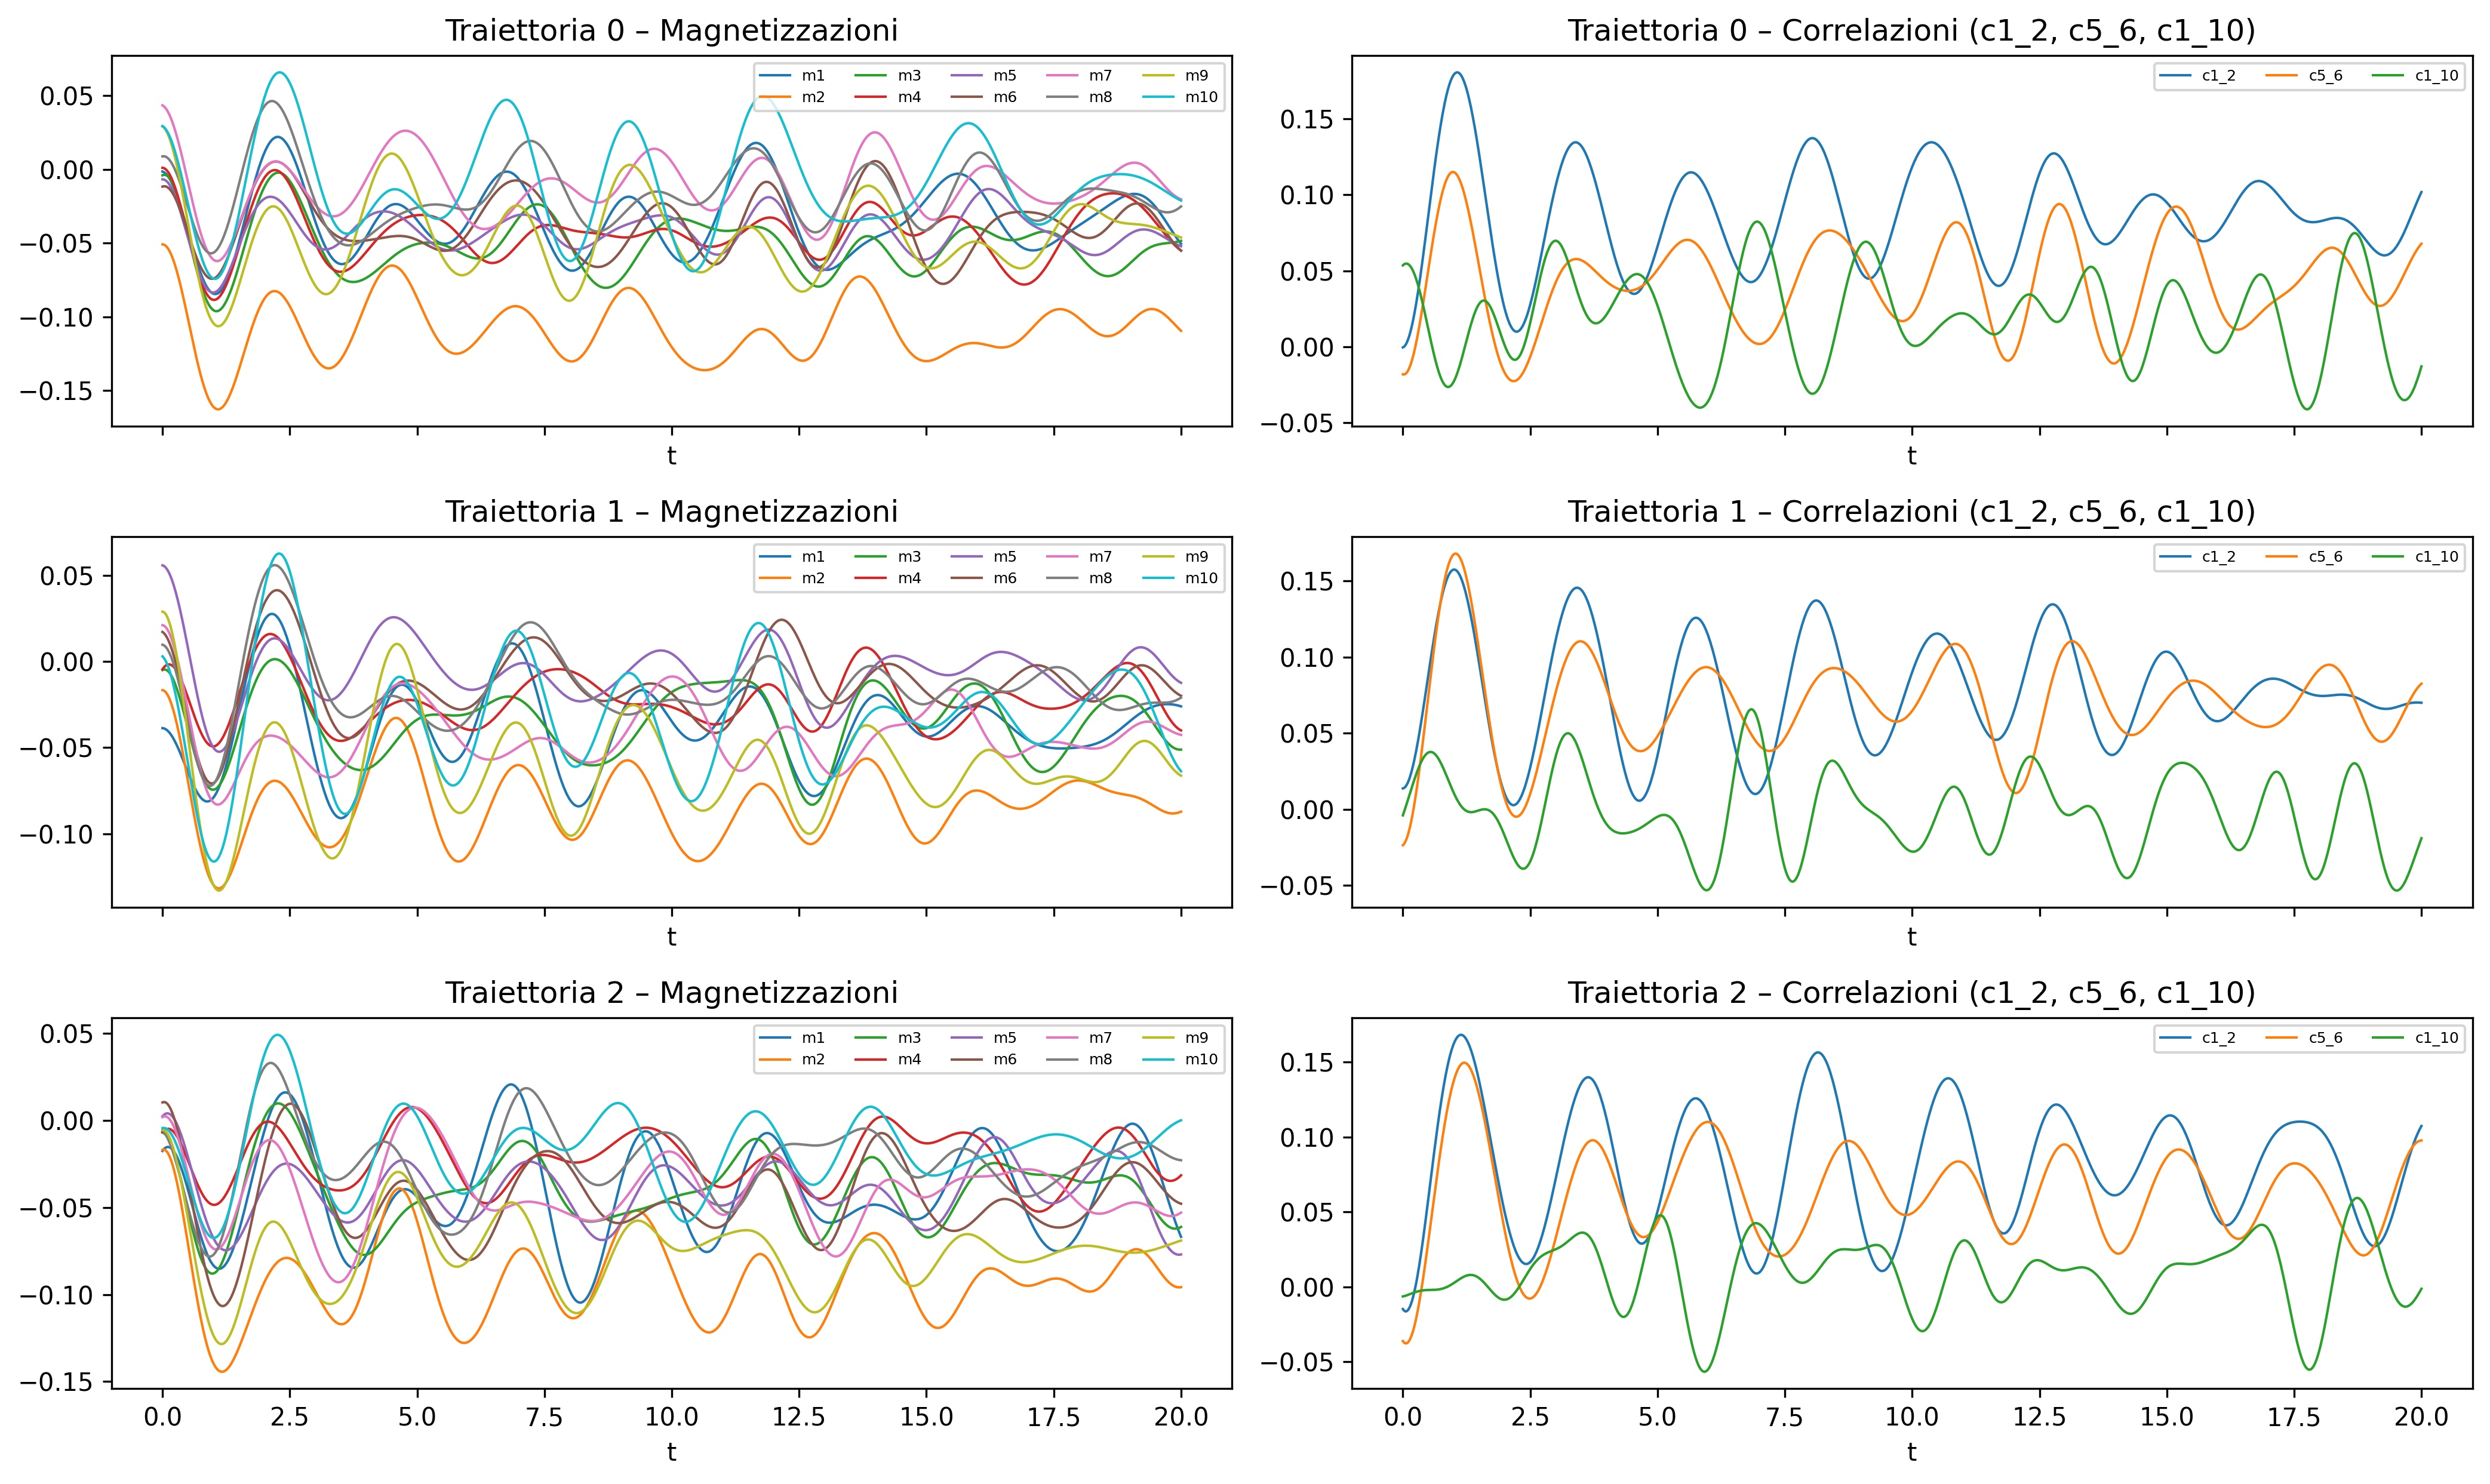
\includegraphics[width=\textwidth,height=3.6cm,keepaspectratio]{figures/01_data/example_trajectories.jpeg}
        \caption{Sample trajectories: magnetizations $m_i$ and correlations $c_{ij}$.}
    \end{subfigure}
    \hfill
    \begin{subfigure}[b]{0.48\textwidth}
        \centering
        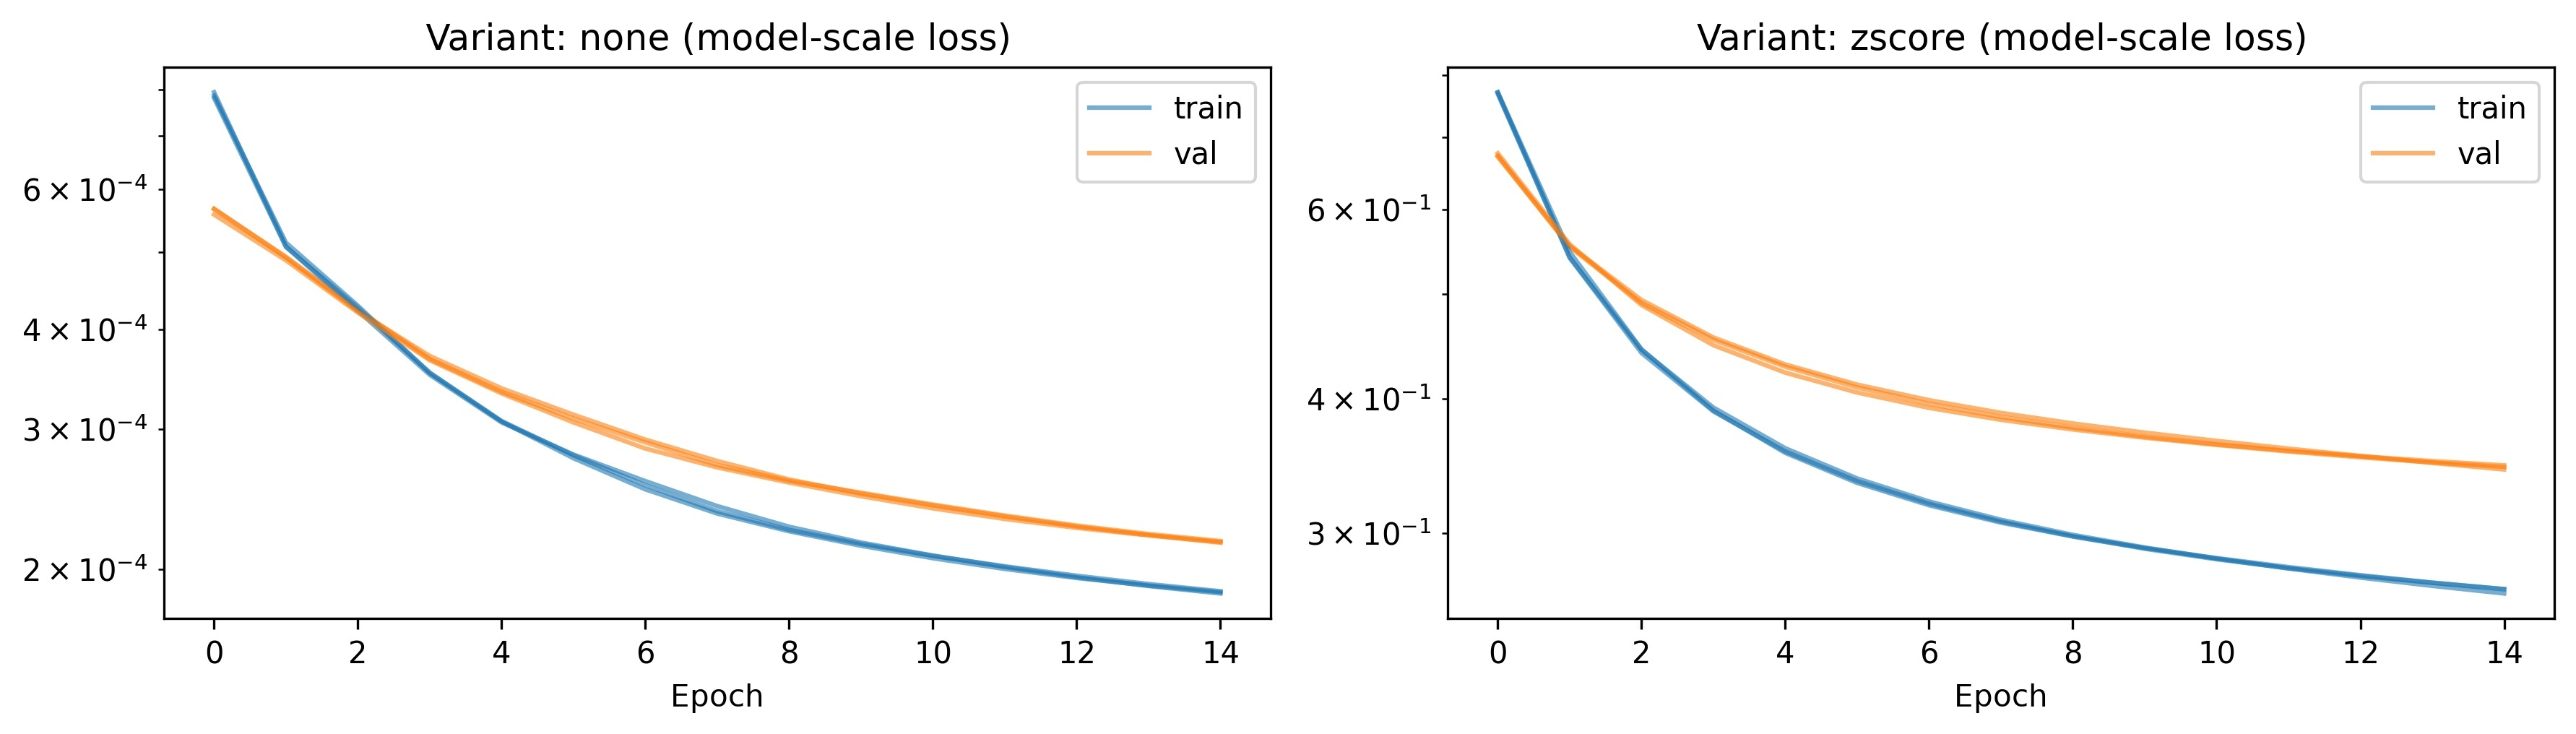
\includegraphics[width=\textwidth,height=3.6cm,keepaspectratio]{figures/01_data/normalization_loss_curves.jpeg}
        \caption{Ablation: raw data ($\tanh$) vs.\ Z-score standardization.}
    \end{subfigure}
    \caption{Physical observables in the 10-qubit PXP chain (left) and 3-seed validation loss curves comparing raw physical inputs with $\tanh$ output against Z-score standardization (right).}
    \label{fig:data_and_norm}
\end{figure}

\subsection{Preprocessing and Windowing}
\textbf{Trajectory-Level Splitting.} Using \texttt{split\_seed = 42}, the $400$ trajectories are partitioned strictly by trajectory ID into $70\%$ training ($280$ trajectories), $15\%$ validation ($60$ trajectories), and $15\%$ test ($60$ trajectories). Splitting whole trajectories rather than slicing windows across trajectories prevents any temporal data leakage (\texttt{check\_no\_leakage} verified across all splits).

\textbf{Normalization Ablation.} Because all $55$ observables are Pauli expectation values bounded in $[-1, 1]$, we conducted a 3-seed ablation (\texttt{seeds = [42, 43, 44]}) comparing raw inputs (\texttt{normalization = "none"}) paired with a bounded $\tanh$ output head against column-wise Z-score standardization (\texttt{zscore}) paired with a linear output head (Table~\ref{tab:norm_ablation} and Fig.~\ref{fig:data_and_norm}b).

\begin{table}[H]
    \centering
    \small
    \caption{Empirical normalization ablation across 3 random seeds (Student-$t$ 95\% CI) on the validation set (\texttt{results/normalization\_comparison.csv}).}
    \label{tab:norm_ablation}
    \resizebox{\textwidth}{!}{%
    \begin{tabular}{llcccccc}
        \toprule
        \textbf{Preprocessing} & \textbf{Output Head} & \textbf{Val MSE ($\times 10^{-4}$)} & \textbf{Val MAE ($\times 10^{-2}$)} & \textbf{Mag MSE ($\times 10^{-4}$)} & \textbf{Corr MSE ($\times 10^{-4}$)} & \textbf{Bounded} & \textbf{Positivity Viol.} \\
        \midrule
        \textbf{Raw Data (\texttt{none})} & \textbf{$\tanh$} & $\mathbf{2.17 \pm 0.01}$ & $\mathbf{1.105 \pm 0.002}$ & $\mathbf{1.11 \pm 0.03}$ & $\mathbf{2.40 \pm 0.02}$ & \textbf{Yes} $[-1, 1]$ & \textbf{0.0\%} \\
        Standardized (\texttt{zscore}) & Linear & $2.32 \pm 0.04$ & $1.135 \pm 0.011$ & $1.33 \pm 0.03$ & $2.54 \pm 0.05$ & No & $0.0\%$ \\
        \bottomrule
    \end{tabular}%
    }
\end{table}

\textbf{Note.} Z-score standardization artificially amplifies low-variance long-range correlations ($|i-j| \ge 3$), injecting noise into gradient updates. Retaining raw physical units with a $\tanh$ activation reduces validation MSE by $6.7\%$ ($2.17 \times 10^{-4}$ vs.\ $2.32 \times 10^{-4}$) and mathematically enforces $\hat{y} \in [-1, 1]$.

\textbf{Sliding Window Generation (\texttt{src/windowing.py}).} We extract windows with stride $s = 10$ across three experimental protocols:
\begin{itemize}[leftmargin=*, itemsep=2pt]
    \item \textbf{Canonical Benchmark Windows:} \texttt{short} ($T_{\text{in}} = 10, T_{\text{out}} = 40$, yielding $26{,}880$ train / $5{,}760$ val / $5{,}760$ test windows) and \texttt{long} ($T_{\text{in}} = 20, T_{\text{out}} = 40$, yielding $26{,}600$ train / $5{,}700$ val / $5{,}700$ test windows).
    \item \textbf{Aligned Challenge 1 Grid:} For $T_{\text{in}} \in \{5, 10, 20, 40\}$, setting \texttt{align\_t\_in = 40} anchors the target window $\mathbf{Y}$ to identical physical time intervals ($26{,}040$ train / $5{,}580$ val / $5{,}580$ test windows for every $T_{\text{in}}$), ensuring a bias-free comparison (Fig.~\ref{fig:windowing}).
    \item \textbf{Challenge 2 Super-Resolution ($\times 2$):} \texttt{make\_sr\_windows} extracts $T_{\text{in}} = 20$ subsampled past steps at $\Delta \tau_{\text{sub}} = 0.04\text{ s}$ ($\mathbf{X}_{\text{sr}} \in \mathbb{R}^{B \times 20 \times 55}$) paired with $T_{\text{out}} = 40$ dense future steps at $\Delta \tau = 0.02\text{ s}$ ($\mathbf{Y}_{\text{sr}} \in \mathbb{R}^{B \times 40 \times 55}$).
\end{itemize}

\begin{figure}[H]
    \centering
    \begin{subfigure}[b]{0.48\textwidth}
        \centering
        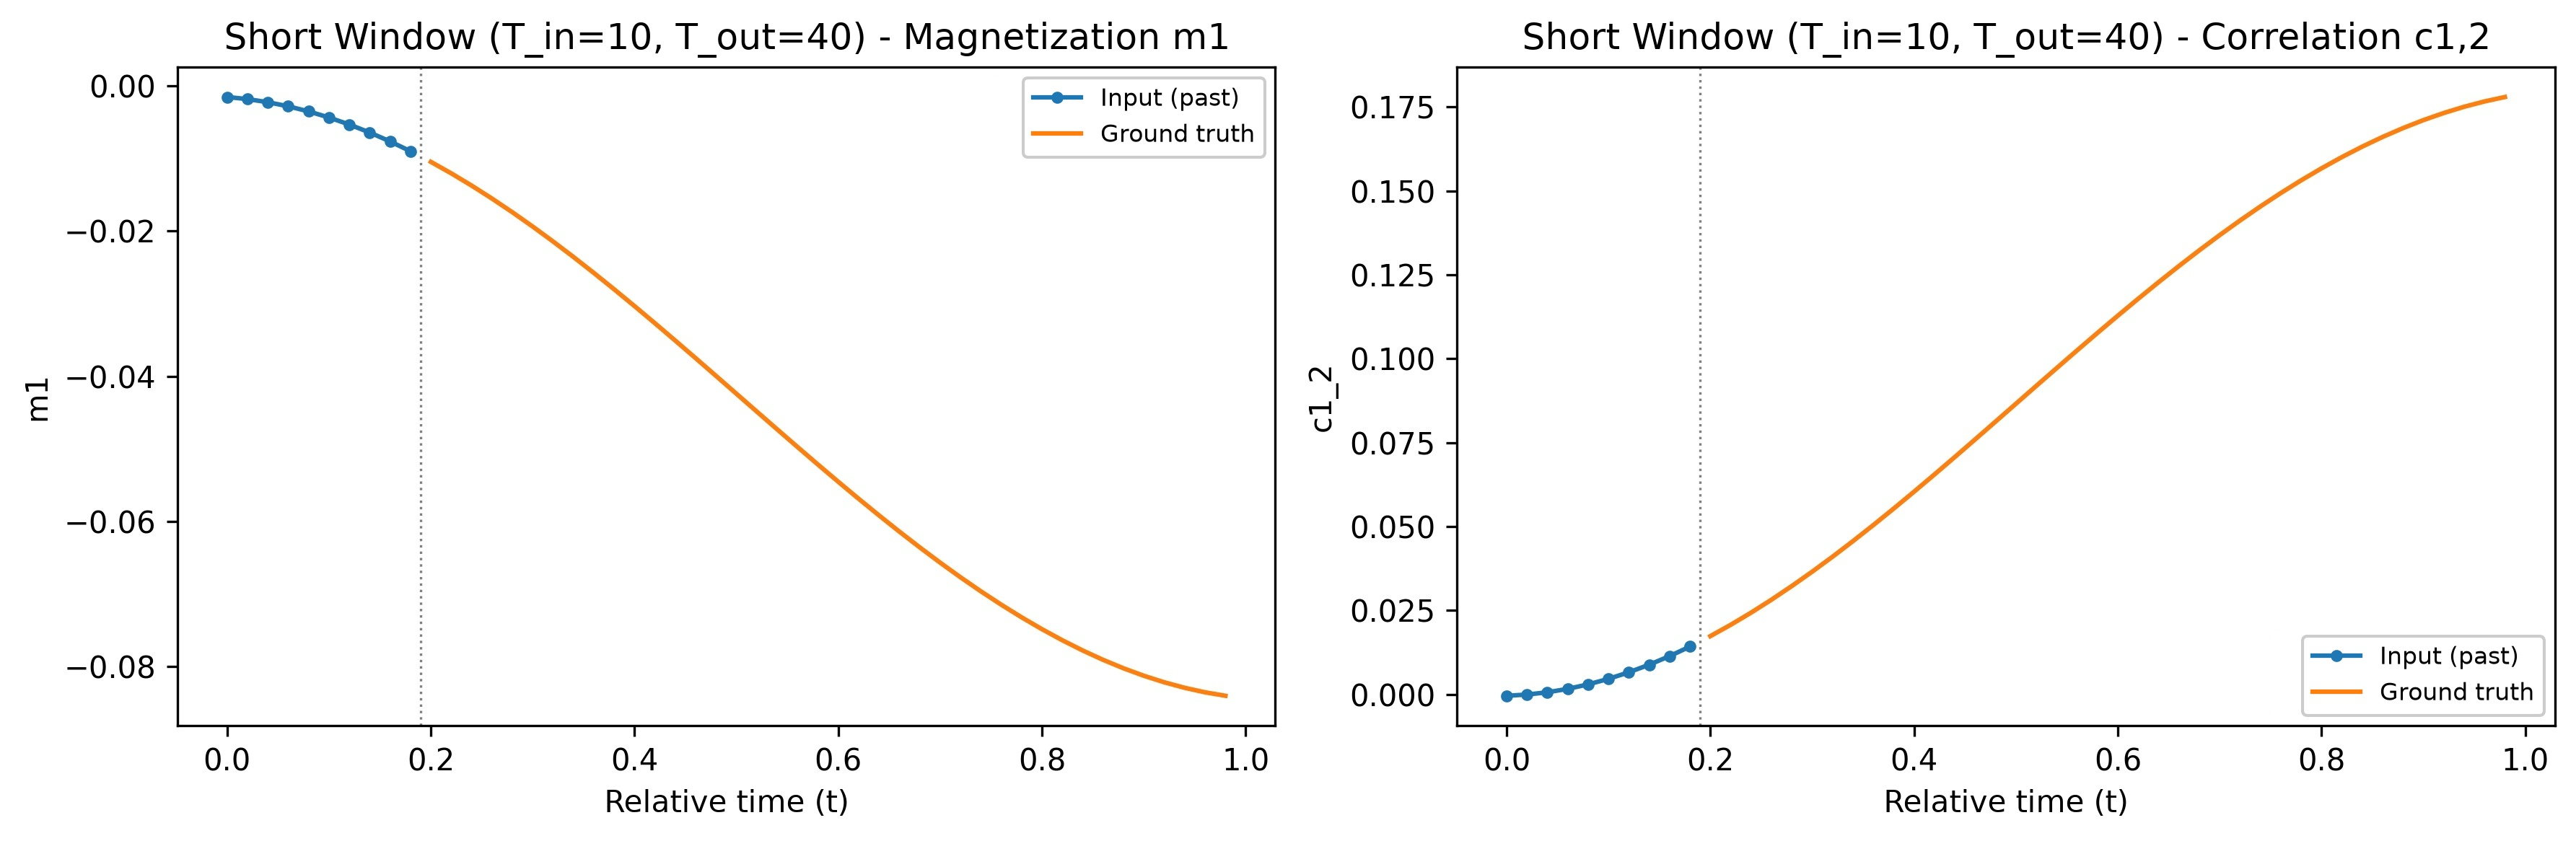
\includegraphics[width=\textwidth,height=3.5cm,keepaspectratio]{figures/02_windowing/window_sample_short.jpeg}
        \caption{Sliding window sample: input $T_{\text{in}}=10$, target $T_{\text{out}}=40$.}
    \end{subfigure}
    \hfill
    \begin{subfigure}[b]{0.48\textwidth}
        \centering
        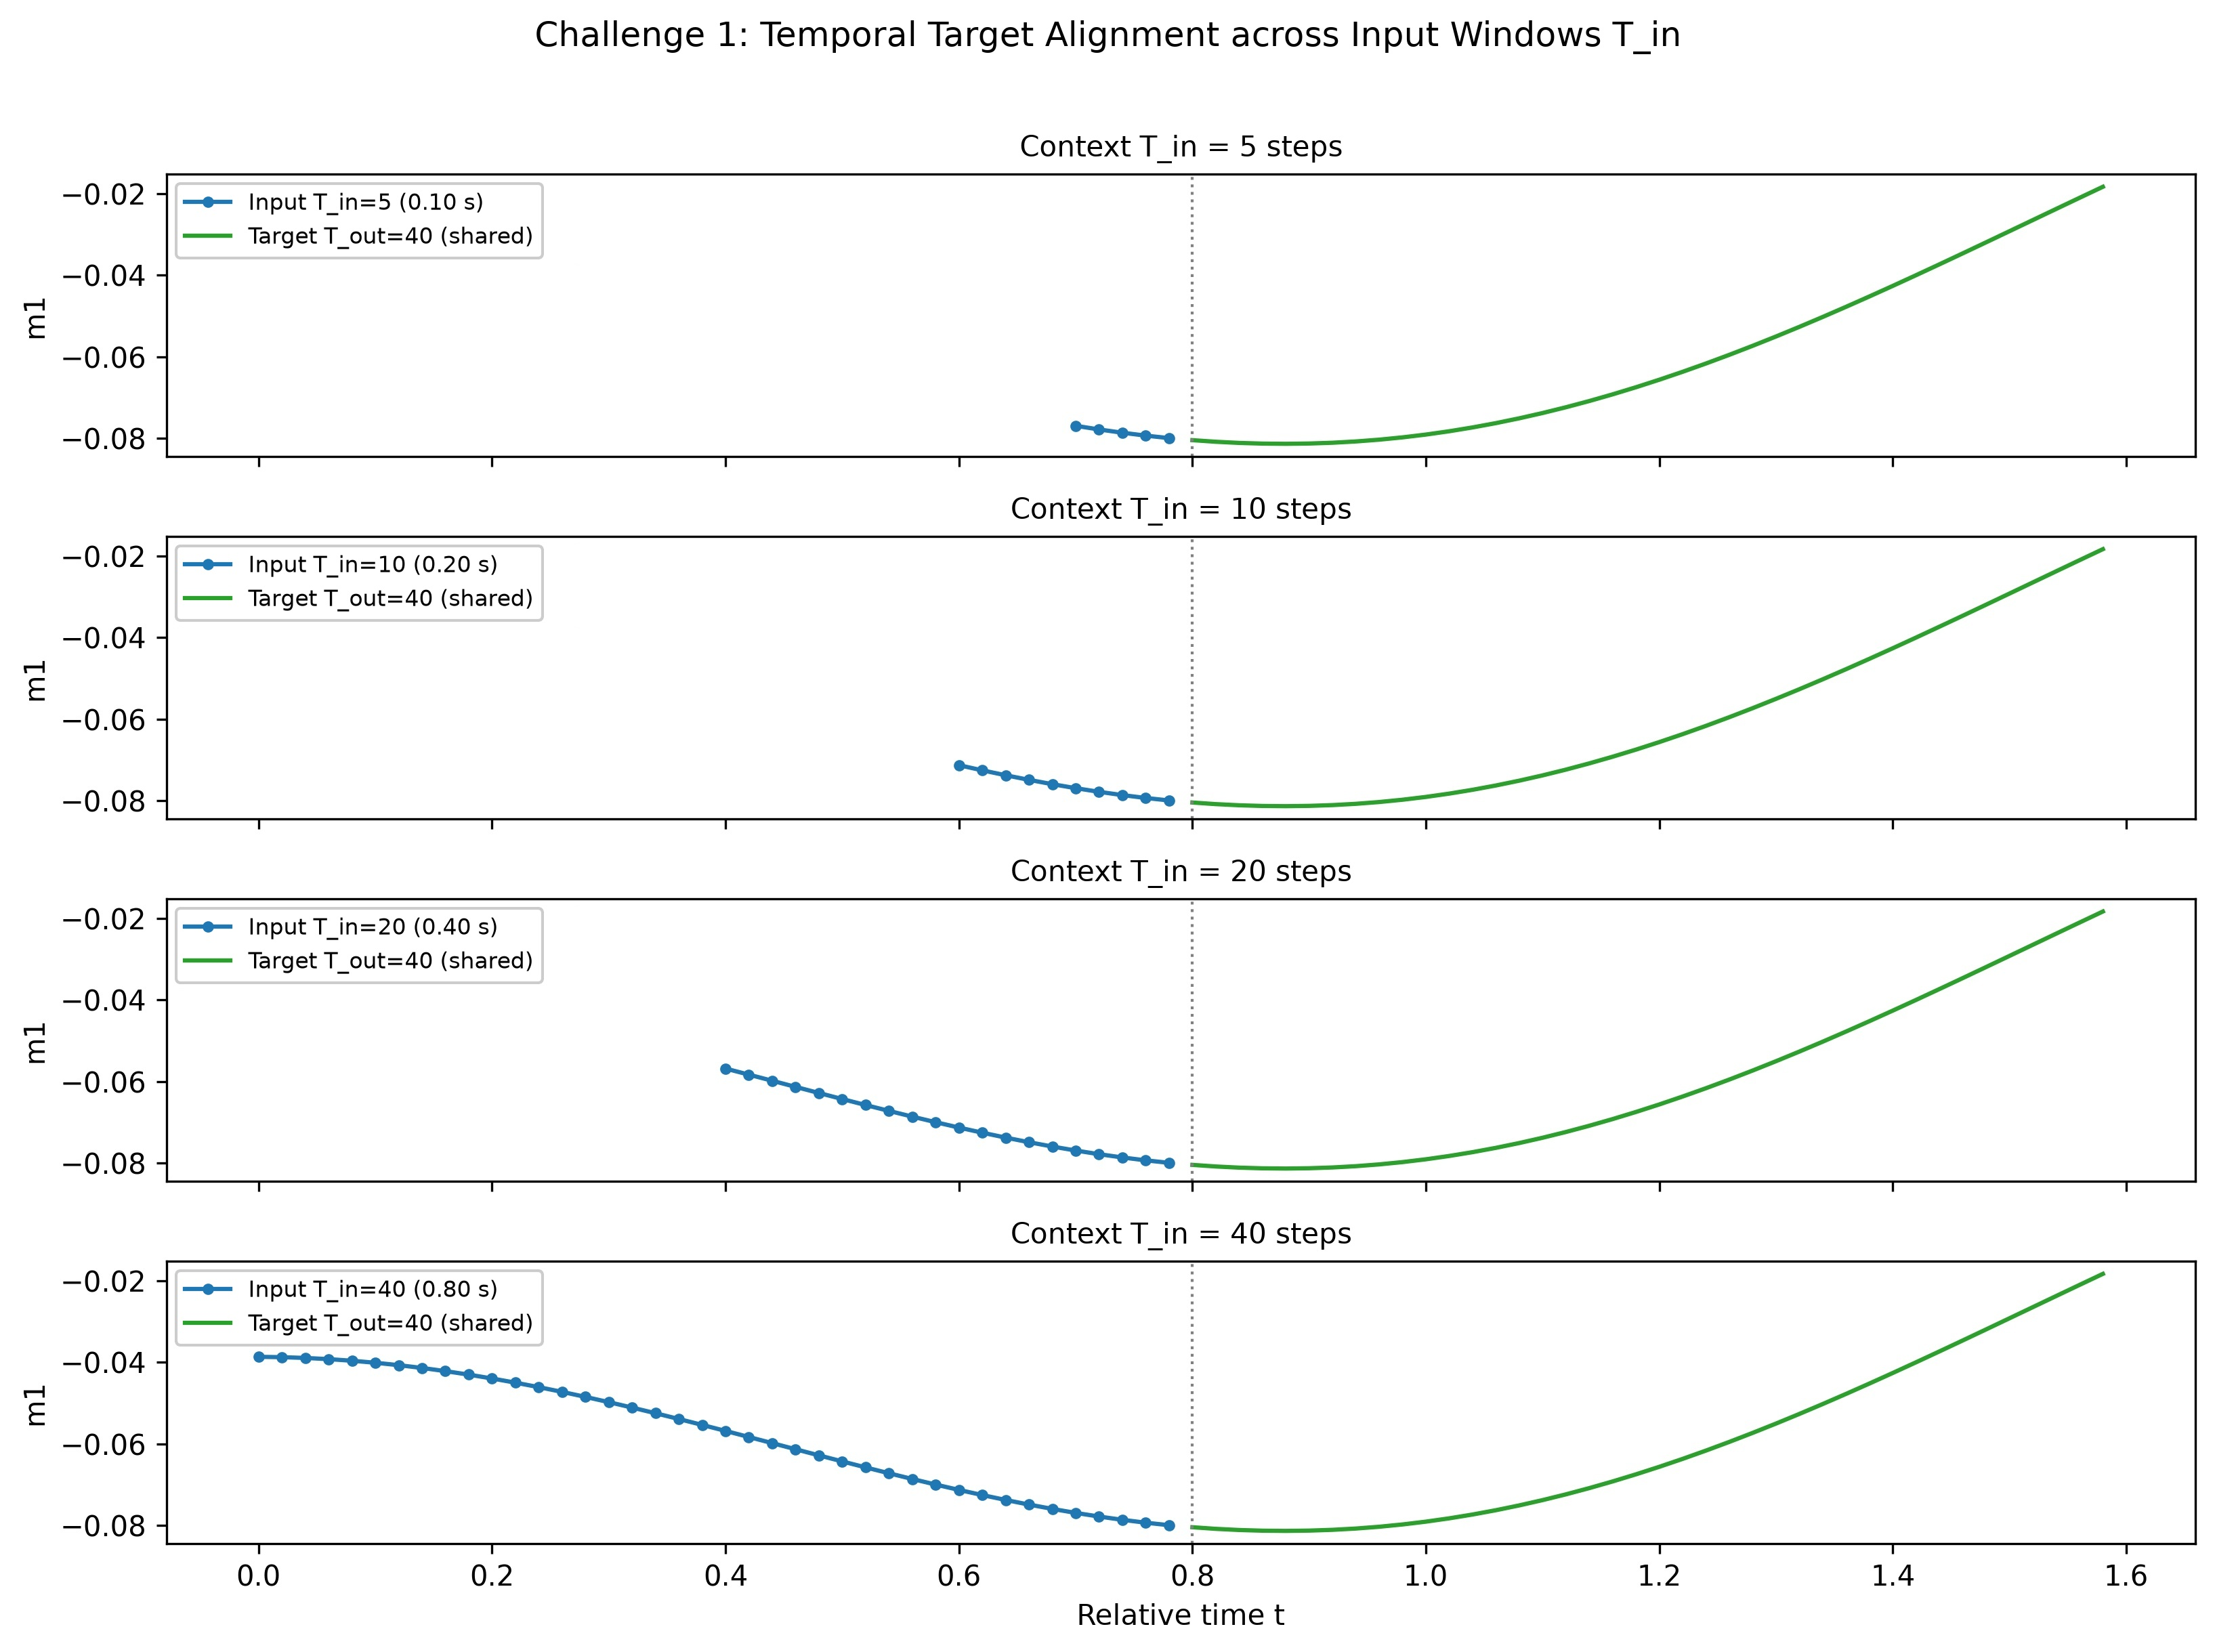
\includegraphics[width=\textwidth,height=3.5cm,keepaspectratio]{figures/02_windowing/tin_grid_comparison.jpeg}
        \caption{Aligned history windows $T_{\text{in}} \in \{5, 10, 20, 40\}$.}
    \end{subfigure}
    \caption{Window extraction for multi-step forecasting (left) and aligned input context comparison for Challenge~1 (right).}
    \label{fig:windowing}
\end{figure}

% =============================================================================
\section{Models and Training Strategy}
% =============================================================================

\subsection{Incremental Progression and Autoencoder Pilot Study}
Following an incremental design philosophy, we began with a \textbf{Start-Small Pilot} on $N_{\text{pilot}} = 20$ trajectories ($1{,}920$ windows) to validate pipeline throughput and convergence before full-scale training (Fig.~\ref{fig:start_small_ae}a).

\textbf{Autoencoder Dimensionality Reduction (Lab 6 Integration).} We also investigated whether compressing the $55$ observables into a $16$-dimensional latent bottleneck ($55 \to 32 \to 16 \to 32 \to 55$) could accelerate sequence learning. While the Latent Transformer reduces parameter count by $60.5\%$ (from $312{,}984$ to $123{,}607$ parameters), the Autoencoder introduces an irreducible pointwise reconstruction floor of $\text{MSE} = 3.62 \times 10^{-4}$. Consequently, latent-space forecasting plateaus at $\text{Val MSE} = 3.74 \times 10^{-4}$ ($3.57 \times 10^{-4}$ on the full dataset), roughly $3\times$ worse than forecasting directly in the 55-D observable space ($1.21 \times 10^{-4}$, Fig.~\ref{fig:start_small_ae}b). All primary models therefore operate directly on the $D = 55$ native observables.

\begin{figure}[H]
    \centering
    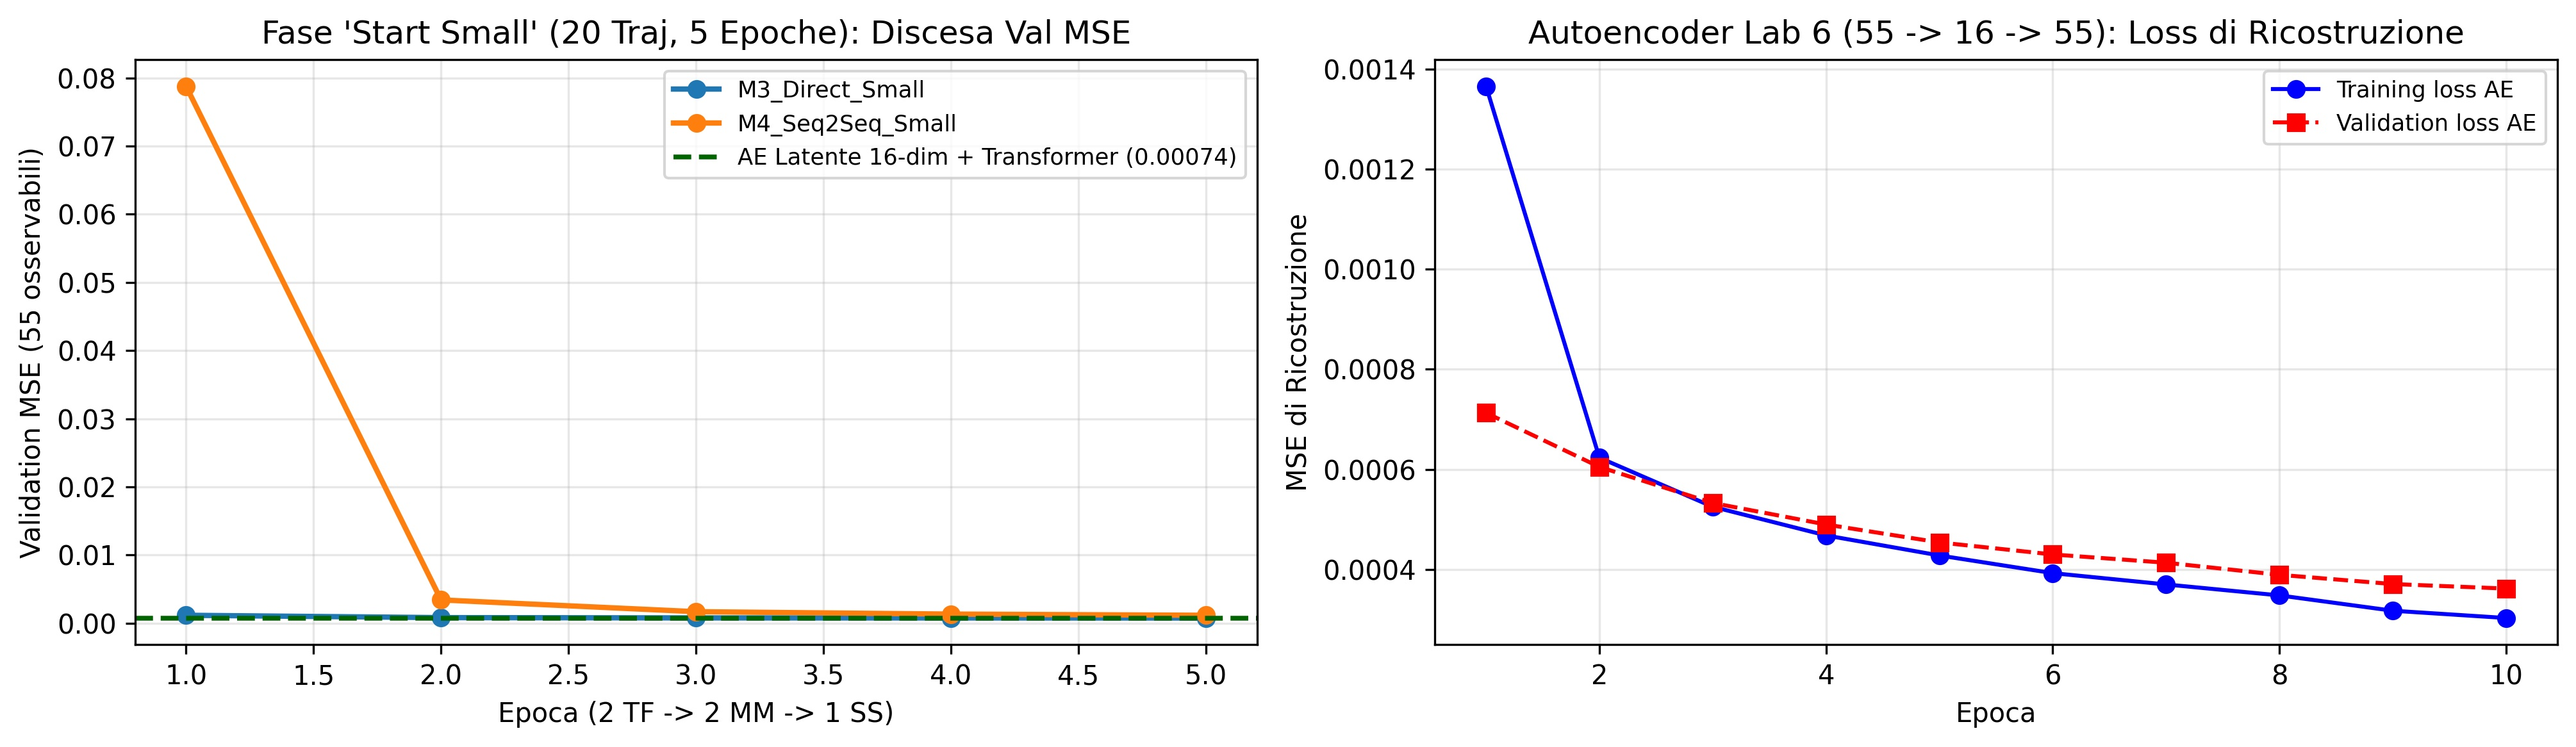
\includegraphics[width=0.84\textwidth,height=3.5cm,keepaspectratio]{figures/04_transformer/start_small_and_autoencoder.jpeg}
    \caption{Start-Small pilot validation curves on 20 trajectories (left) and Lab~6 Autoencoder reconstruction floor vs.\ native 55-D Transformer forecasting (right).}
    \label{fig:start_small_ae}
\end{figure}

\subsection{Model Architectures}
\textbf{Notation:} $B$ = batch size ($64$), $T_{\text{in}}$ = input length, $T_{\text{out}} = 40$ = forecasting horizon, $D = 55$ = physical observables, $d_{\text{rnn}}$ = recurrent hidden units, $d_{\text{model}}$ = Transformer embedding dimension, $d_{\text{ff}}$ = feed-forward dimension, $H$ = attention heads, $L$ = stacked layers. All hyperparameters are managed through a centralized configuration dictionary (\texttt{DEFAULT\_CONFIG} and \texttt{make\_config} in \texttt{src/config.py}).

We implemented and compared four sequence architectures across Recurrent (\texttt{src/models\_rnn.py}) and Lab~7 Transformer (\texttt{src/models\_transformer.py}) families:
\begin{itemize}[leftmargin=*, itemsep=2pt]
    \item \textbf{M1 --- Direct One-Shot RNN (\texttt{build\_rnn\_direct}):} Stacked cuDNN-accelerated LSTM or GRU encoder layers compress the input window $(B, T_{\text{in}}, 55)$ into a final hidden vector $\mathbf{h}_{T_{\text{in}}} \in \mathbb{R}^{B \times d_{\text{rnn}}}$; a single-shot dense head $\text{Dense}(T_{\text{out}} \times 55, \tanh)$ followed by $\text{Reshape}(T_{\text{out}}, 55)$ predicts the entire 40-step horizon simultaneously without recursive feedback.
    \item \textbf{M2 --- Autoregressive Seq2Seq RNN (\texttt{RNNSeq2Seq}):} Encoder-decoder LSTM/GRU transferring full internal states $(\mathbf{h}_\ell, \mathbf{c}_\ell)_{\ell=1}^L$ from encoder to decoder. Trained with shifted decoder inputs in parallel (\texttt{call}) and evaluated step-by-step in closed loop (\texttt{predict\_free\_running}).
    \item \textbf{M3 --- Direct One-Shot Transformer (\texttt{TransformerDirect}):} Encoder-only Transformer adapting the Lab~7 architecture to continuous time series via \texttt{PositionalEmbedding} ($\text{Dense}(d_{\text{model}}) \cdot \sqrt{d_{\text{model}}} + \text{PE}$) and $L$ \texttt{EncoderLayer} blocks (\texttt{GlobalSelfAttention} + \texttt{FeedForward} with Post-LN residual connections). The contextualized final time step $\mathbf{z}_{T_{\text{in}}} = \text{Encoder}(\mathbf{X})[:, -1, :] \in \mathbb{R}^{B \times d_{\text{model}}}$ is projected in one shot via $\text{Dense}(T_{\text{out}} \times 55, \tanh) + \text{Reshape}(T_{\text{out}}, 55)$.
    \item \textbf{M4 --- Causal Seq2Seq Transformer (\texttt{TransformerSeq2Seq}):} Full Lab~7 Encoder-Decoder Transformer. Each \texttt{DecoderLayer} applies \texttt{CausalSelfAttention} (\texttt{use\_causal\_mask=True}), \texttt{CrossAttention} attending to encoder memory $M$, and \texttt{FeedForward}, followed by \texttt{Dense(55, tanh)}. Exposes \texttt{get\_attention\_scores} in eager mode for Challenge~3 interpretability.
\end{itemize}

\begin{table}[H]
    \centering
    \small
    \caption{Architectural specification of Recurrent models (M1 Direct and M2 Seq2Seq) and Transformer models (M3 Direct and M4 Seq2Seq).}
    \label{tab:architectures}
    \resizebox{\textwidth}{!}{%
    \begin{tabular}{llll}
        \toprule
        \textbf{Model Family} & \textbf{Stage / Module} & \textbf{Layer / Operation} & \textbf{Output Tensor Shape} \\
        \midrule
        \multirow{2}{*}{\textbf{M1 (Direct RNN)}} & Encoder & $L \times \text{LSTM/GRU}(d_{\text{rnn}})$ + Inter-layer Dropout & $(B, d_{\text{rnn}})$ \\
        & One-Shot Head & $\text{Dense}(T_{\text{out}} \cdot D, \tanh) \to \text{Reshape}(T_{\text{out}}, D)$ & $(B, T_{\text{out}}, 55)$ \\
        \midrule
        \multirow{2}{*}{\textbf{M2 (Seq2Seq RNN)}} & Encoder & $L \times \text{LSTM/GRU}(d_{\text{rnn}}, \text{return\_state=True})$ & States $\{(\mathbf{h}_\ell, \mathbf{c}_\ell)\}_{\ell=1}^L$ \\
        & Autoregressive Decoder & $L \times \text{LSTM/GRU}(d_{\text{rnn}}) \to \text{Dropout} \to \text{Dense}(D, \tanh)$ & $(B, T_{\text{out}}, 55)$ \\
        \midrule
        \multirow{3}{*}{\textbf{M3 (Direct Transformer)}} & Input Embedding & $\text{Dense}(d_{\text{model}}) \cdot \sqrt{d_{\text{model}}} + \text{Sinusoidal PE} + \text{Dropout}$ & $(B, T_{\text{in}}, d_{\text{model}})$ \\
        & Encoder Stack & $L \times [\text{GlobalSelfAttention}(H, d_{\text{model}}) + \text{FFN}(d_{\text{ff}})]$ & $(B, T_{\text{in}}, d_{\text{model}})$ \\
        & One-Shot Head & Slice $\mathbf{z}_{T_{\text{in}}}[:, -1, :] \to \text{Dense}(T_{\text{out}} \cdot D, \tanh) \to \text{Reshape}$ & $(B, T_{\text{out}}, 55)$ \\
        \midrule
        \multirow{3}{*}{\textbf{M4 (Seq2Seq Transformer)}} & Encoder Stack & $\text{PositionalEmbedding} \to L \times \text{EncoderLayer}$ & Memory $M: (B, T_{\text{in}}, d_{\text{model}})$ \\
        & Causal Decoder Stack & $\text{PositionalEmbedding} \to L \times [\text{CausalMHA} + \text{CrossAttn}(M) + \text{FFN}]$ & $(B, T_{\text{out}}, d_{\text{model}})$ \\
        & Stepwise Head & $\text{Dense}(D, \tanh)$ (parallel in TF / iterative in Free-Running) & $(B, T_{\text{out}}, 55)$ \\
        \bottomrule
    \end{tabular}%
    }
\end{table}

\subsection{Three-Phase Hybrid Training Curriculum and Free-Running Evaluation}
To ensure a rigorous comparison across all 24 benchmark models, every architecture is trained for \textbf{25 epochs} (\texttt{batch\_size = 64}, Adam optimizer with $\text{lr} = 10^{-3}$, MSE loss) using our unified three-phase training loop (\texttt{train\_hybrid} in \texttt{src/training.py}):

\begin{table}[H]
    \centering
    \small
    \caption{Three-phase hybrid training curriculum implemented in \texttt{src/training.py} (\texttt{train\_hybrid}).}
    \label{tab:training_phases}
    \resizebox{\textwidth}{!}{%
    \begin{tabular}{llcl}
        \toprule
        \textbf{Phase} & \textbf{Epochs} & \textbf{Config Parameters} & \textbf{Operational Mechanism in Direct (M1, M3) and Seq2Seq (M2, M4) Models} \\
        \midrule
        \textbf{1. Teacher Forcing (\texttt{tf})} & $1\text{--}10$ ($10$) & \texttt{epochs\_tf = 10} & Unmasked encoder input $\mathbf{X}$; Seq2Seq decoder receives ground-truth shifted targets $\mathbf{Y}_{\text{shift}}$ ($p_{\text{ss}} = 0$). \\
        \textbf{2. Masked Modeling (\texttt{mm})} & $11\text{--}20$ ($10$) & \texttt{mask\_ratio = 0.15} & Randomly zeroes $15\%$ of time steps (\texttt{mask\_timesteps}), protecting anchor step $t_0$ to enforce non-local interpolation. \\
        \textbf{3. Scheduled Sampling (\texttt{ss})} & $21\text{--}25$ ($5$) & $p_{\text{ss}}: 0.0 \to 0.5$ & Two-pass parallel sampling~\cite{bengio2015,mihaylova2019}: mixes self-generated predictions $\hat{\mathbf{Y}}$ into decoder inputs (\texttt{mix\_decoder\_inputs}). \\
        \bottomrule
    \end{tabular}%
    }
\end{table}

\textbf{Realistic Free-Running Validation and Checkpoint Restoration.} During training, Teacher Forcing loss can be overly optimistic for autoregressive models because the decoder receives ground-truth history. In \texttt{train\_hybrid}, validation MSE (\texttt{val\_mse}) is computed at the end of \textbf{every single epoch} using true unassisted inference (\texttt{predict\_free\_running} compiled with \texttt{@tf.function(reduce\_retracing=True)} for M2 and M4, and one-shot forward pass for M1 and M3). Across all 25 epochs, \texttt{train\_hybrid} tracks the lowest free-running validation MSE and automatically restores the optimal weights (\texttt{restore\_best = True}).

\subsection{Hyperparameter Tuning Grid}
We designed a systematic two-level full factorial grid comprising $4$ architectures $\times$ $3$ capacity configurations (HP1, HP2, HP3) $\times$ $2$ input windows (\texttt{short}, \texttt{long}) $= 24$ benchmark runs:
\begin{itemize}[leftmargin=*, itemsep=2pt]
    \item \textbf{Recurrent Family (M1, M2):} \textbf{HP1} = 1-layer LSTM, $64$ units, dropout $0.0$; \textbf{HP2} = 2-layer stacked LSTM, $64$ units, dropout $0.1$; \textbf{HP3} = 1-layer GRU, $64$ units, dropout $0.0$.
    \item \textbf{Transformer Family (M3, M4):} \textbf{HP1} = 2 layers, $d_{\text{model}}=64$, $H=4$ heads, $d_{\text{ff}}=128$, dropout $0.1$; \textbf{HP2} = 2 layers, $d_{\text{model}}=128$, $H=4$ heads, $d_{\text{ff}}=256$, dropout $0.1$; \textbf{HP3} = 1 layer, $d_{\text{model}}=64$, $H=2$ heads, $d_{\text{ff}}=128$, dropout $0.0$.
\end{itemize}

% =============================================================================
\section{Experimental Results}
% =============================================================================

\subsection{Training Dynamics and Exposure Bias Analysis}
Figure~\ref{fig:loss_and_free_running}a illustrates validation MSE trajectories across the 25-epoch hybrid curriculum (\texttt{tf} $\to$ \texttt{mm} $\to$ \texttt{ss}). Direct one-shot models (M1, M3) converge smoothly and benefit from Masked Modeling regularization in epochs 11--20. By contrast, autoregressive Seq2Seq models (M2, M4) experience a pronounced validation floor in free-running mode due to recursive error propagation.

\begin{figure}[H]
    \centering
    \begin{subfigure}[b]{0.48\textwidth}
        \centering
        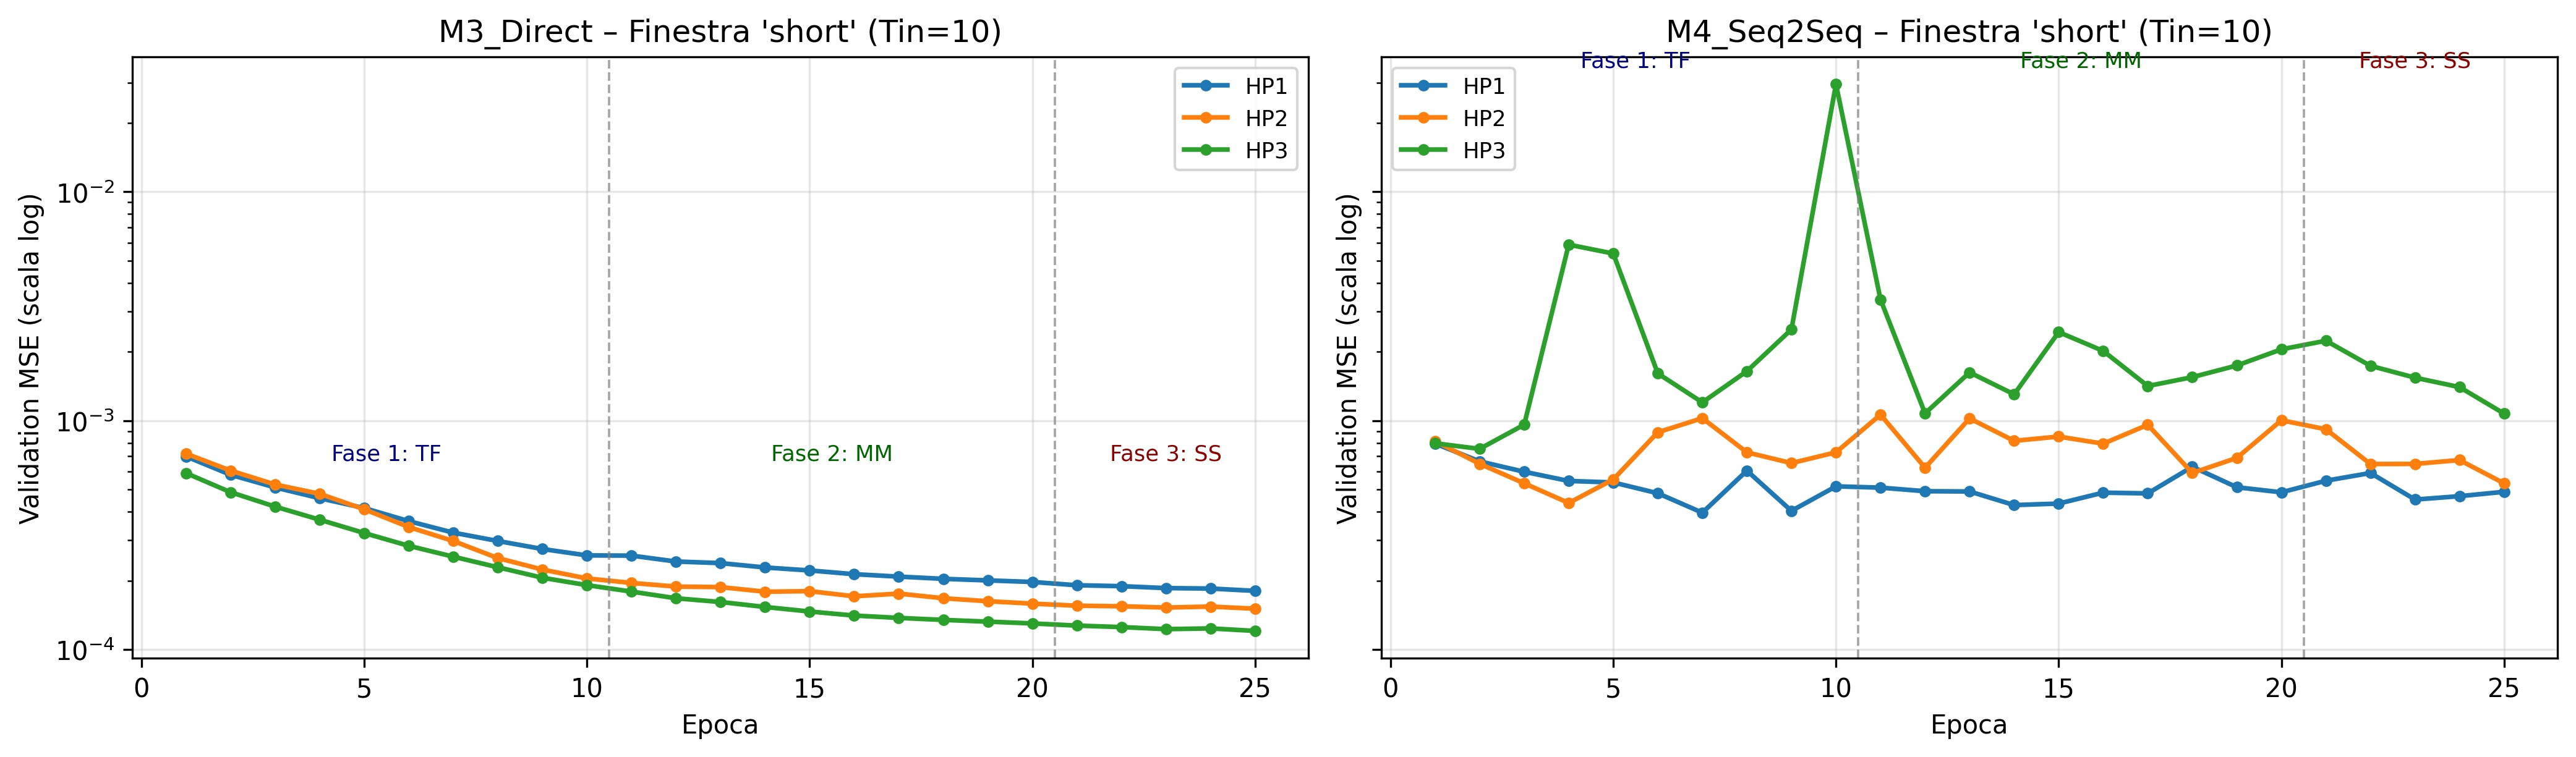
\includegraphics[width=\textwidth,height=3.4cm,keepaspectratio]{figures/04_transformer/loss_curves_hybrid.jpeg}
        \caption{Validation MSE across the 3-phase hybrid curriculum.}
    \end{subfigure}
    \hfill
    \begin{subfigure}[b]{0.48\textwidth}
        \centering
        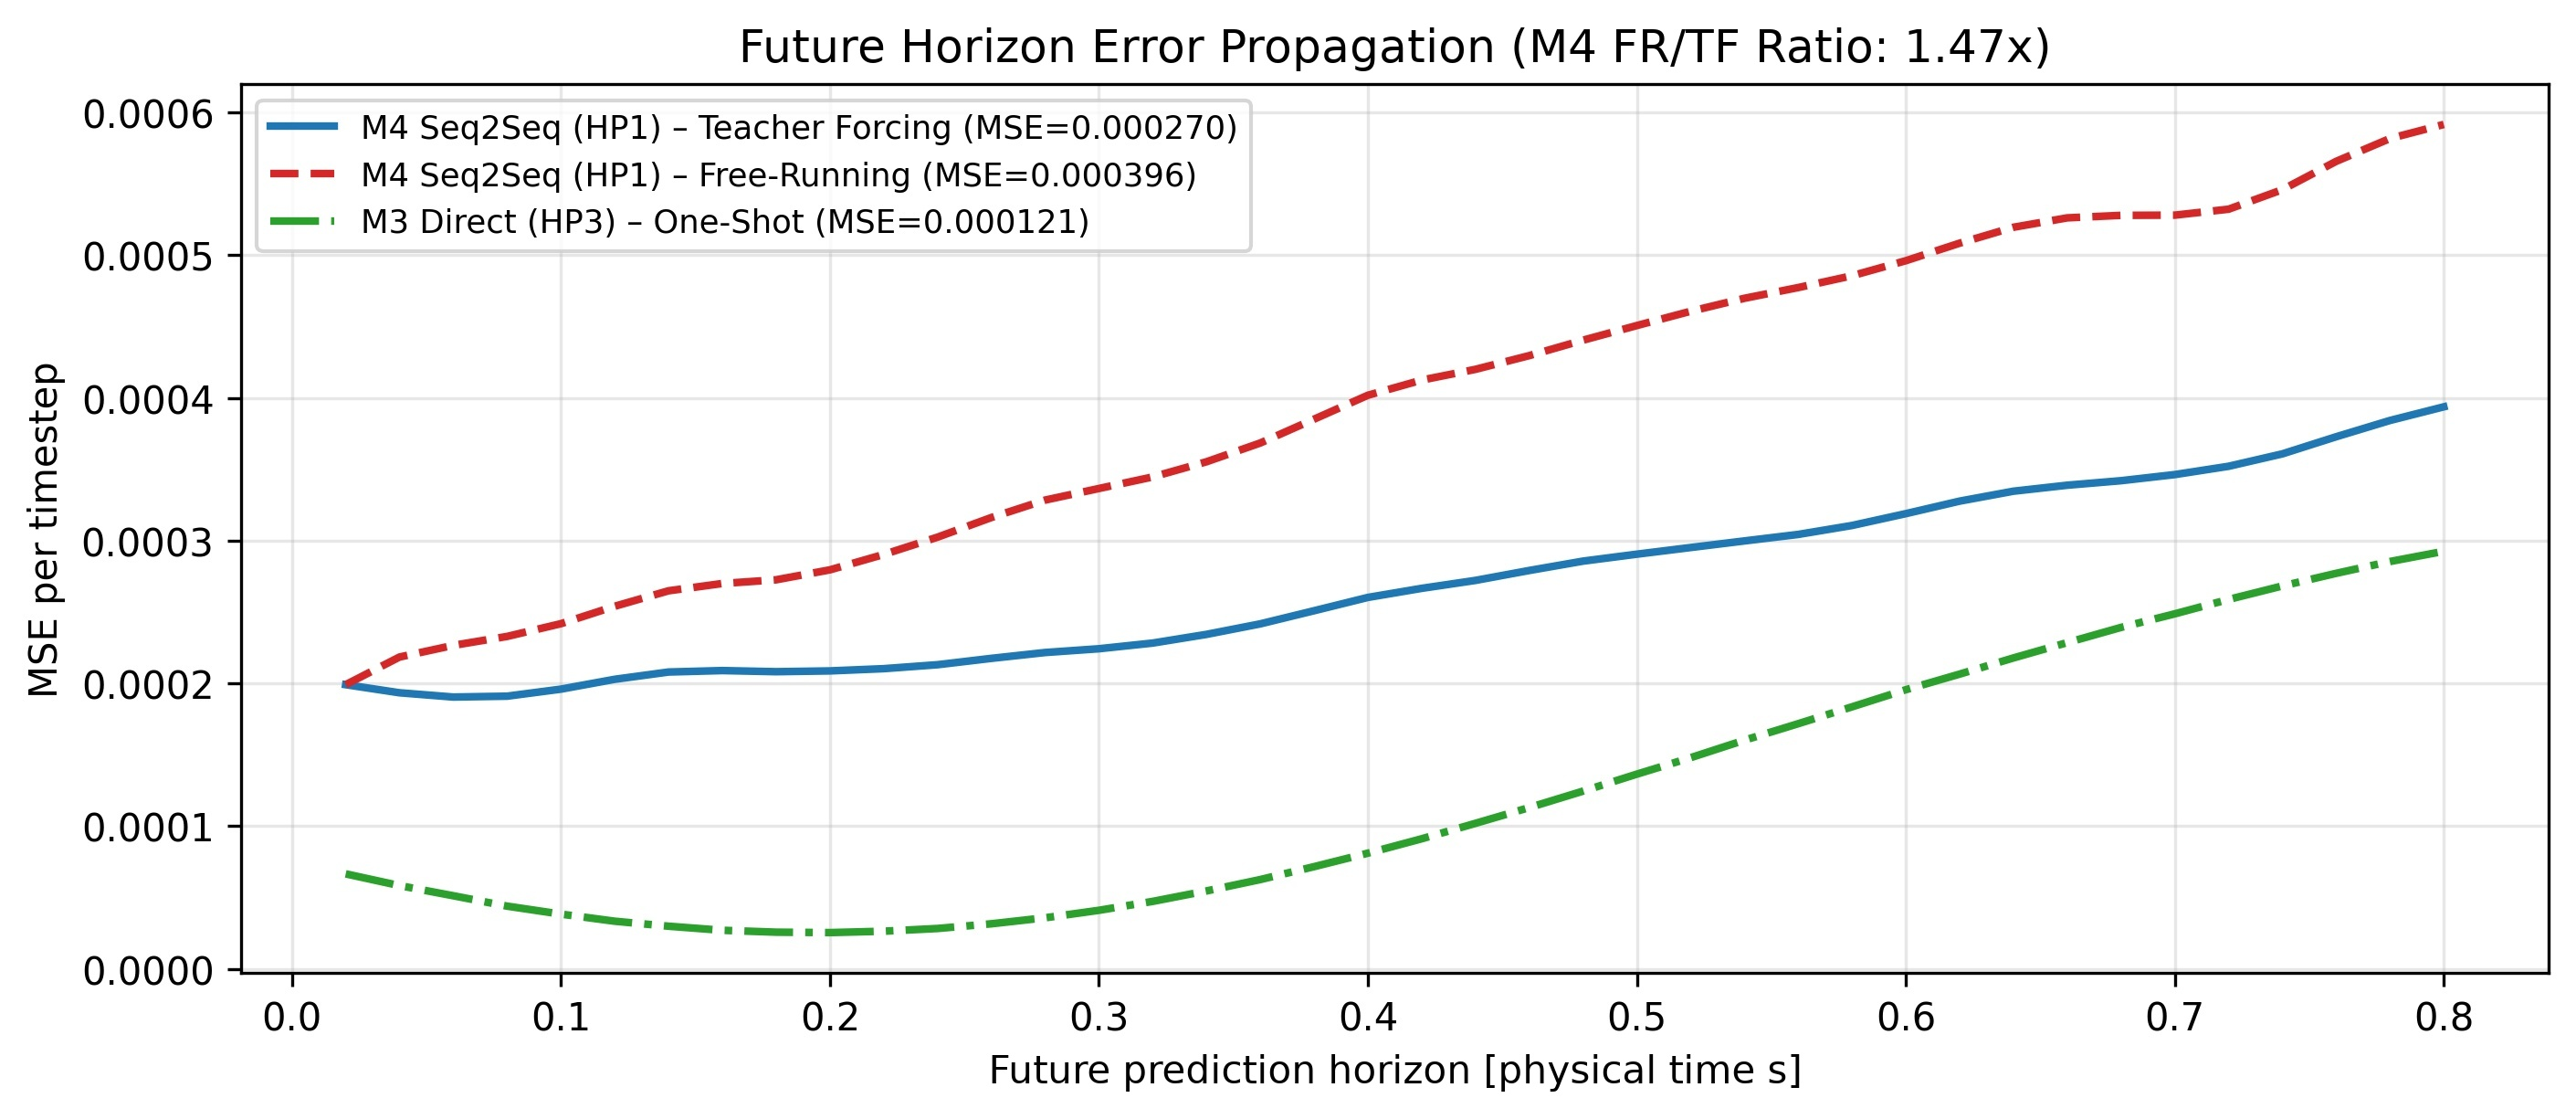
\includegraphics[width=\textwidth,height=3.4cm,keepaspectratio]{figures/04_transformer/free_running_error_accumulation.jpeg}
        \caption{Step-by-step MSE growth across horizon $t \in [1, 40]$.}
    \end{subfigure}
    \caption{Hybrid training curves (left) and step-by-step error accumulation comparing Teacher Forcing, Free-Running M4, and One-Shot M3 (right).}
    \label{fig:loss_and_free_running}
\end{figure}

\textbf{Quantifying Exposure Bias.} Figure~\ref{fig:loss_and_free_running}b dissects step-by-step prediction error across the 40 future steps for M4 (\texttt{TransformerSeq2Seq} HP1) versus M3 (\texttt{TransformerDirect} HP3). When M4 is fed ground-truth tokens under Teacher Forcing, its average MSE is $0.58 \times 10^{-4}$; however, in true unassisted Free-Running inference, small errors at $t = 1$ ($1.99 \times 10^{-4}$) compound recursively into $5.91 \times 10^{-4}$ by $t = 40$ (global Free-Running MSE $= 3.96 \times 10^{-4}$, a $6.8\times$ degradation ratio). One-shot projection in M3 completely eliminates recursive feedback, maintaining a bounded error profile ($0.67 \times 10^{-4}$ at $t=1$ to $2.93 \times 10^{-4}$ at $t=40$, mean $1.21 \times 10^{-4}$).

\subsection{Canonical Benchmark Comparison and 5-Fold Cross-Validation}
Table~\ref{tab:canonical_comparison} presents the canonical Table~1 comparison between the Direct Recurrent family (\textbf{M1 HP1--HP3}) and Direct Transformer family (\textbf{M3 HP1--HP3}), along with 3-seed $95\%$ Student-$t$ confidence intervals ($t_{0.975,2} = 4.303$), 5-fold trajectory cross-validation (\texttt{results/kfold\_cv\_results.csv}), and blind test set evaluation. Table~\ref{tab:full_grid_24} reports the complete 24-model factorial grid (\texttt{results/table1\_benchmark\_complete.csv}).

\begin{table}[H]
    \centering
    \small
    \caption{Canonical benchmark comparison of Direct Recurrent (M1) and Direct Transformer (M3) architectures across HP1--HP3 (\texttt{short} window $T_{\text{in}}=10$, plus \texttt{long} window $T_{\text{in}}=20$, 5-Fold CV, and Blind Test Set). Bold indicates row winner.}
    \label{tab:canonical_comparison}
    \resizebox{\textwidth}{!}{%
    \begin{tabular}{lcccccc}
        \toprule
        \textbf{Metric} & \textbf{M1 (HP1)} & \textbf{M1 (HP2)} & \textbf{M1 (HP3)} & \textbf{M3 (HP1)} & \textbf{M3 (HP2)} & \textbf{M3 (HP3)} \\
        \midrule
        Architecture Config & 1L LSTM 64u & 2L LSTM 64u & 1L GRU 64u & 2L $d=64, H=4$ & 2L $d=128, H=4$ & \textbf{1L $d=64, H=2$} \\
        Model Parameters & $173{,}720$ & $206{,}744$ & $166{,}232$ & $312{,}984$ & $951{,}448$ & $196{,}632$ \\
        Training Time (25 epochs, s) & $47.8$ & $64.0$ & $\mathbf{44.4}$ & $122.5$ & $132.5$ & $73.0$ \\
        \midrule
        Val MSE \texttt{short} ($\times 10^{-4}$) & $1.61 \pm 0.00$ & $1.74$ & $1.63$ & $1.81$ & $1.51$ & $\mathbf{1.21 \pm 0.01}$ \\
        Val MAE \texttt{short} ($\times 10^{-2}$) & $0.912 \pm 0.004$ & $0.973$ & $0.913$ & $1.004$ & $0.894$ & $\mathbf{0.787 \pm 0.010}$ \\
        Val RMSE \texttt{short} ($\times 10^{-2}$) & $1.268$ & $1.319$ & $1.275$ & $1.344$ & $1.229$ & $\mathbf{1.099}$ \\
        \midrule
        Val MSE: Magnetizations ($\times 10^{-4}$) & $0.75$ & $0.81$ & $0.76$ & $0.86$ & $0.57$ & $\mathbf{0.36}$ \\
        Val MSE: Correlations ($\times 10^{-4}$) & $1.80$ & $1.95$ & $1.82$ & $2.02$ & $1.72$ & $\mathbf{1.40}$ \\
        Val MSE at Step $t = 1$ ($\times 10^{-4}$) & $0.04$ & $0.18$ & $\mathbf{0.03}$ & $0.43$ & $0.21$ & $0.67$ \\
        Val MSE at Step $t = 40$ ($\times 10^{-4}$) & $3.24$ & $3.27$ & $3.28$ & $3.33$ & $3.04$ & $\mathbf{2.93}$ \\
        \midrule
        Val MSE \texttt{long} ($T_{\text{in}} = 20$, $\times 10^{-4}$) & $1.47$ & $1.57$ & $1.59$ & $1.69$ & $1.46$ & $\mathbf{1.21}$ \\
        Seq2Seq Counterpart (M2 / M4, $\times 10^{-4}$) & $3.05$ & $2.66$ & $3.41$ & $3.96$ & $4.37$ & $7.53$ \\
        5-Fold CV Val MSE ($\times 10^{-4}$) & $1.60 \pm 0.02$ & --- & --- & --- & --- & $\mathbf{1.20 \pm 0.02}$ \\
        \midrule
        Blind Test MSE ($\times 10^{-4}$) & $1.61$ & --- & --- & --- & --- & $\mathbf{1.21}$ \\
        Blind Test MAE ($\times 10^{-2}$) & $0.911$ & --- & --- & --- & --- & $\mathbf{0.785}$ \\
        Test Positivity Violations ($P < 0$) & $\mathbf{0.0\%}$ ($P_{\min}=0.167$) & --- & --- & --- & --- & $\mathbf{0.0\%}$ ($P_{\min}=0.163$) \\
        \bottomrule
    \end{tabular}%
    }
\end{table}

\textbf{Key Insights from the Benchmark:}
\begin{enumerate}[leftmargin=*, itemsep=2pt]
    \item \textbf{Compact Transformer Superiority:} The compact 1-layer Transformer \textbf{M3 (HP3)} ($196{,}632$ parameters, $d_{\text{model}}=64, H=2$) achieves the best accuracy across both \texttt{short} and \texttt{long} windows ($\text{Val MSE} = 1.21 \times 10^{-4}$, $\text{Test MSE} = 1.21 \times 10^{-4}$), reducing error by $\mathbf{-24.9\%}$ relative to the best RNN \textbf{M1 (HP1)} ($1.61 \times 10^{-4}$). Deeper 2-layer Transformers (HP1: $313\text{k}$ params; HP2: $951\text{k}$ params) overfit slightly compared to the 1-layer HP3 configuration.
    \item \textbf{5-Fold Cross-Validation Stability:} Across 5 trajectory-level folds on the $340$ development trajectories ($272$ train / $68$ val per fold, Fig.~\ref{fig:benchmark_summary}b), M3 (HP3) achieves $\text{Val MSE} = 1.20 \times 10^{-4} \pm 0.02 \times 10^{-4}$ ($\text{MAE} = 0.00781 \pm 0.00010$), outperforming M1 (HP1) ($1.60 \times 10^{-4} \pm 0.02 \times 10^{-4}$) on every fold with non-overlapping $95\%$ confidence intervals.
\end{enumerate}

\begin{figure}[H]
    \centering
    \begin{subfigure}[b]{0.48\textwidth}
        \centering
        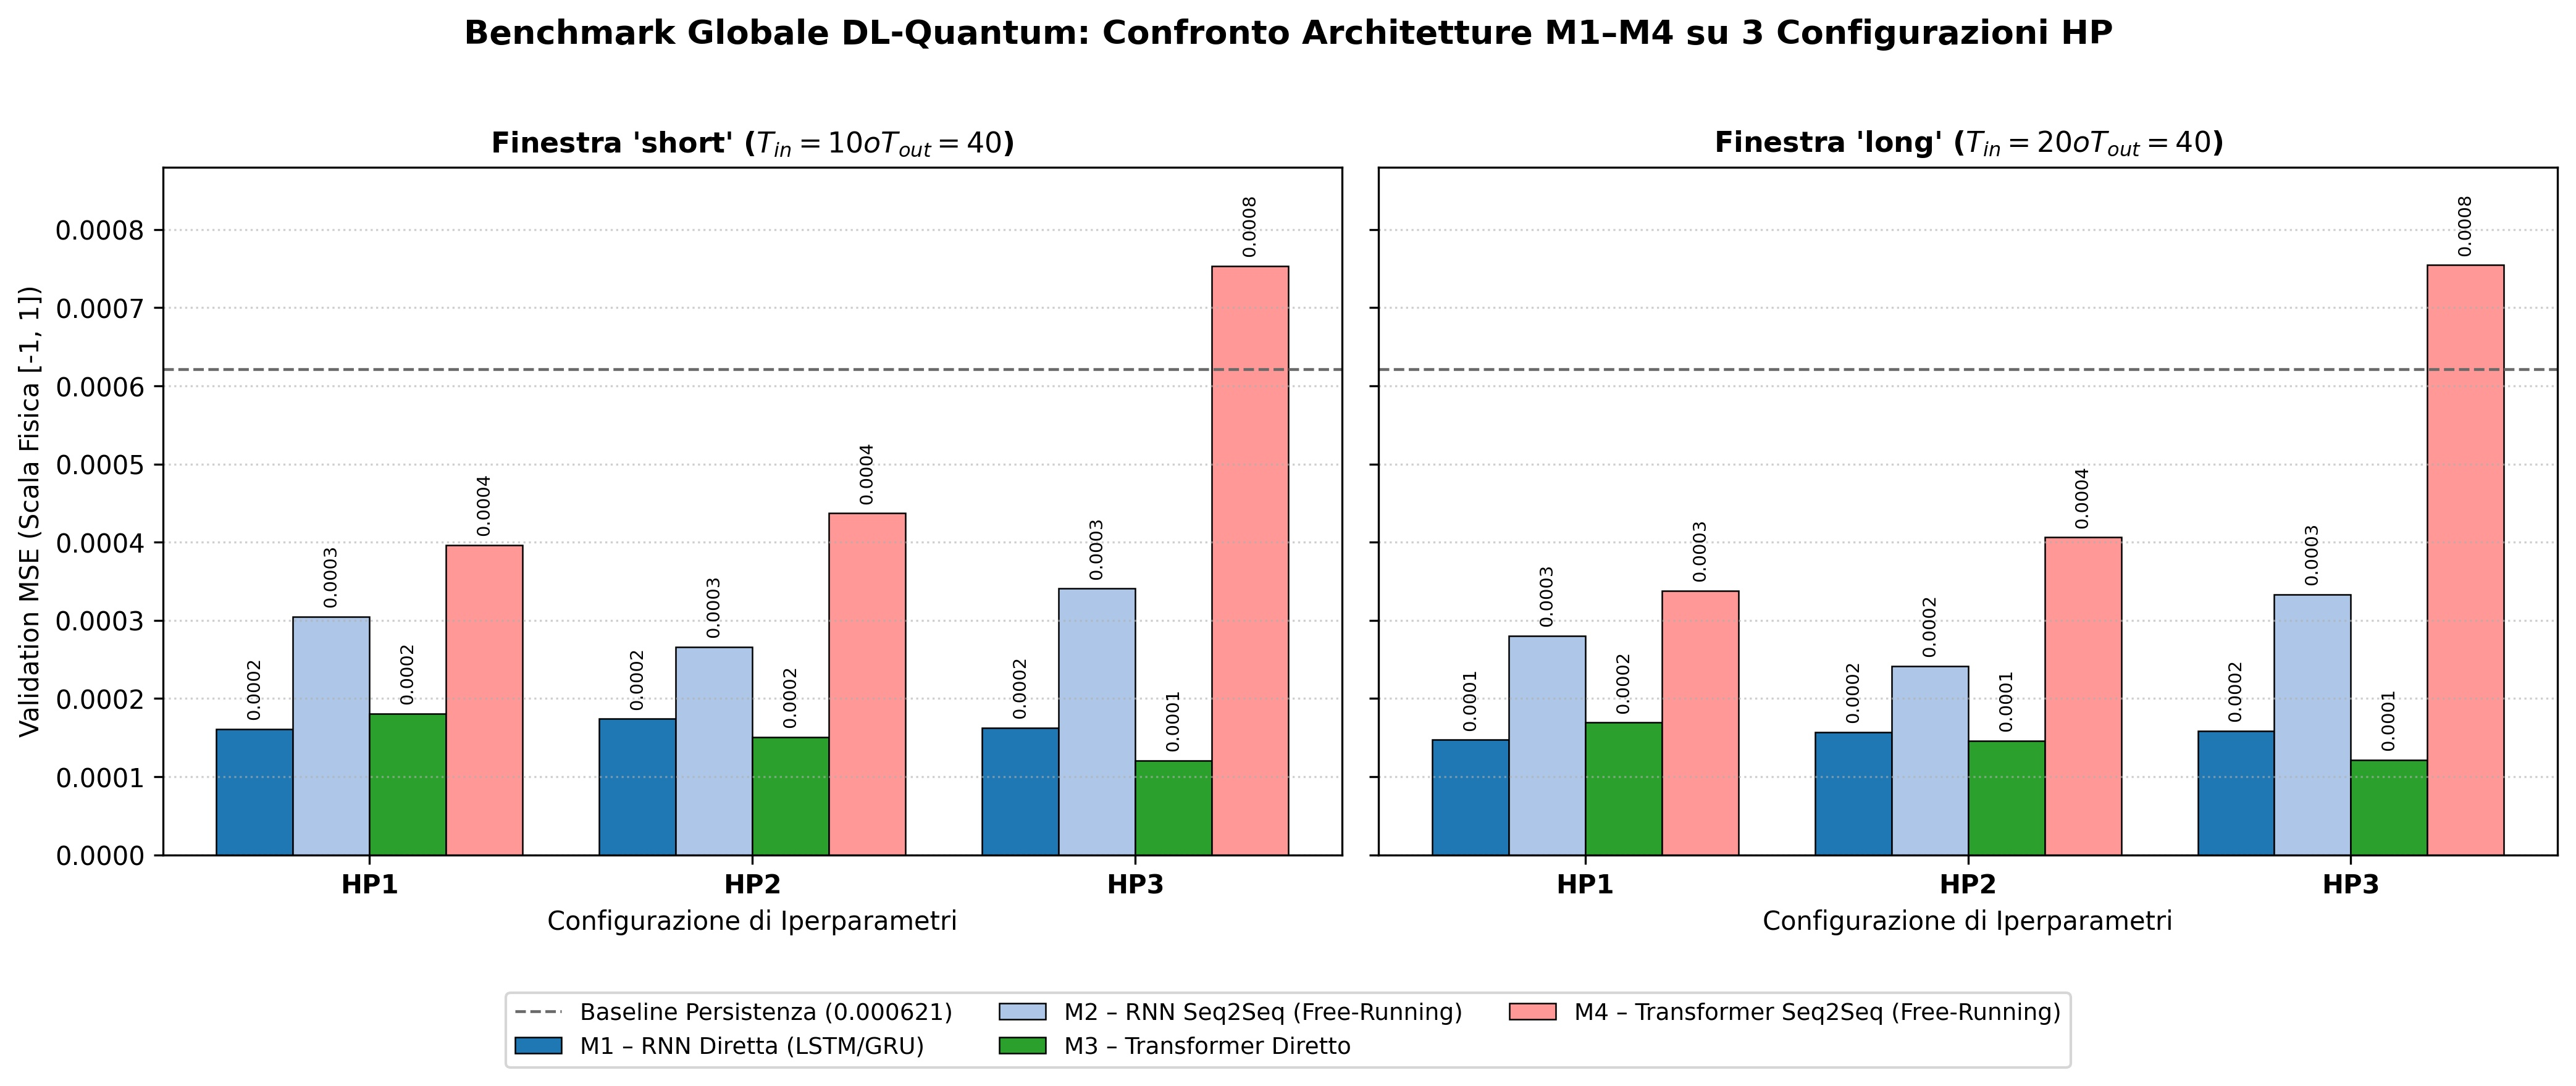
\includegraphics[width=\textwidth,height=3.5cm,keepaspectratio]{figures/05_inference/global_benchmark_summary.jpeg}
        \caption{24-model benchmark: Validation MSE across \texttt{short} and \texttt{long}.}
    \end{subfigure}
    \hfill
    \begin{subfigure}[b]{0.48\textwidth}
        \centering
        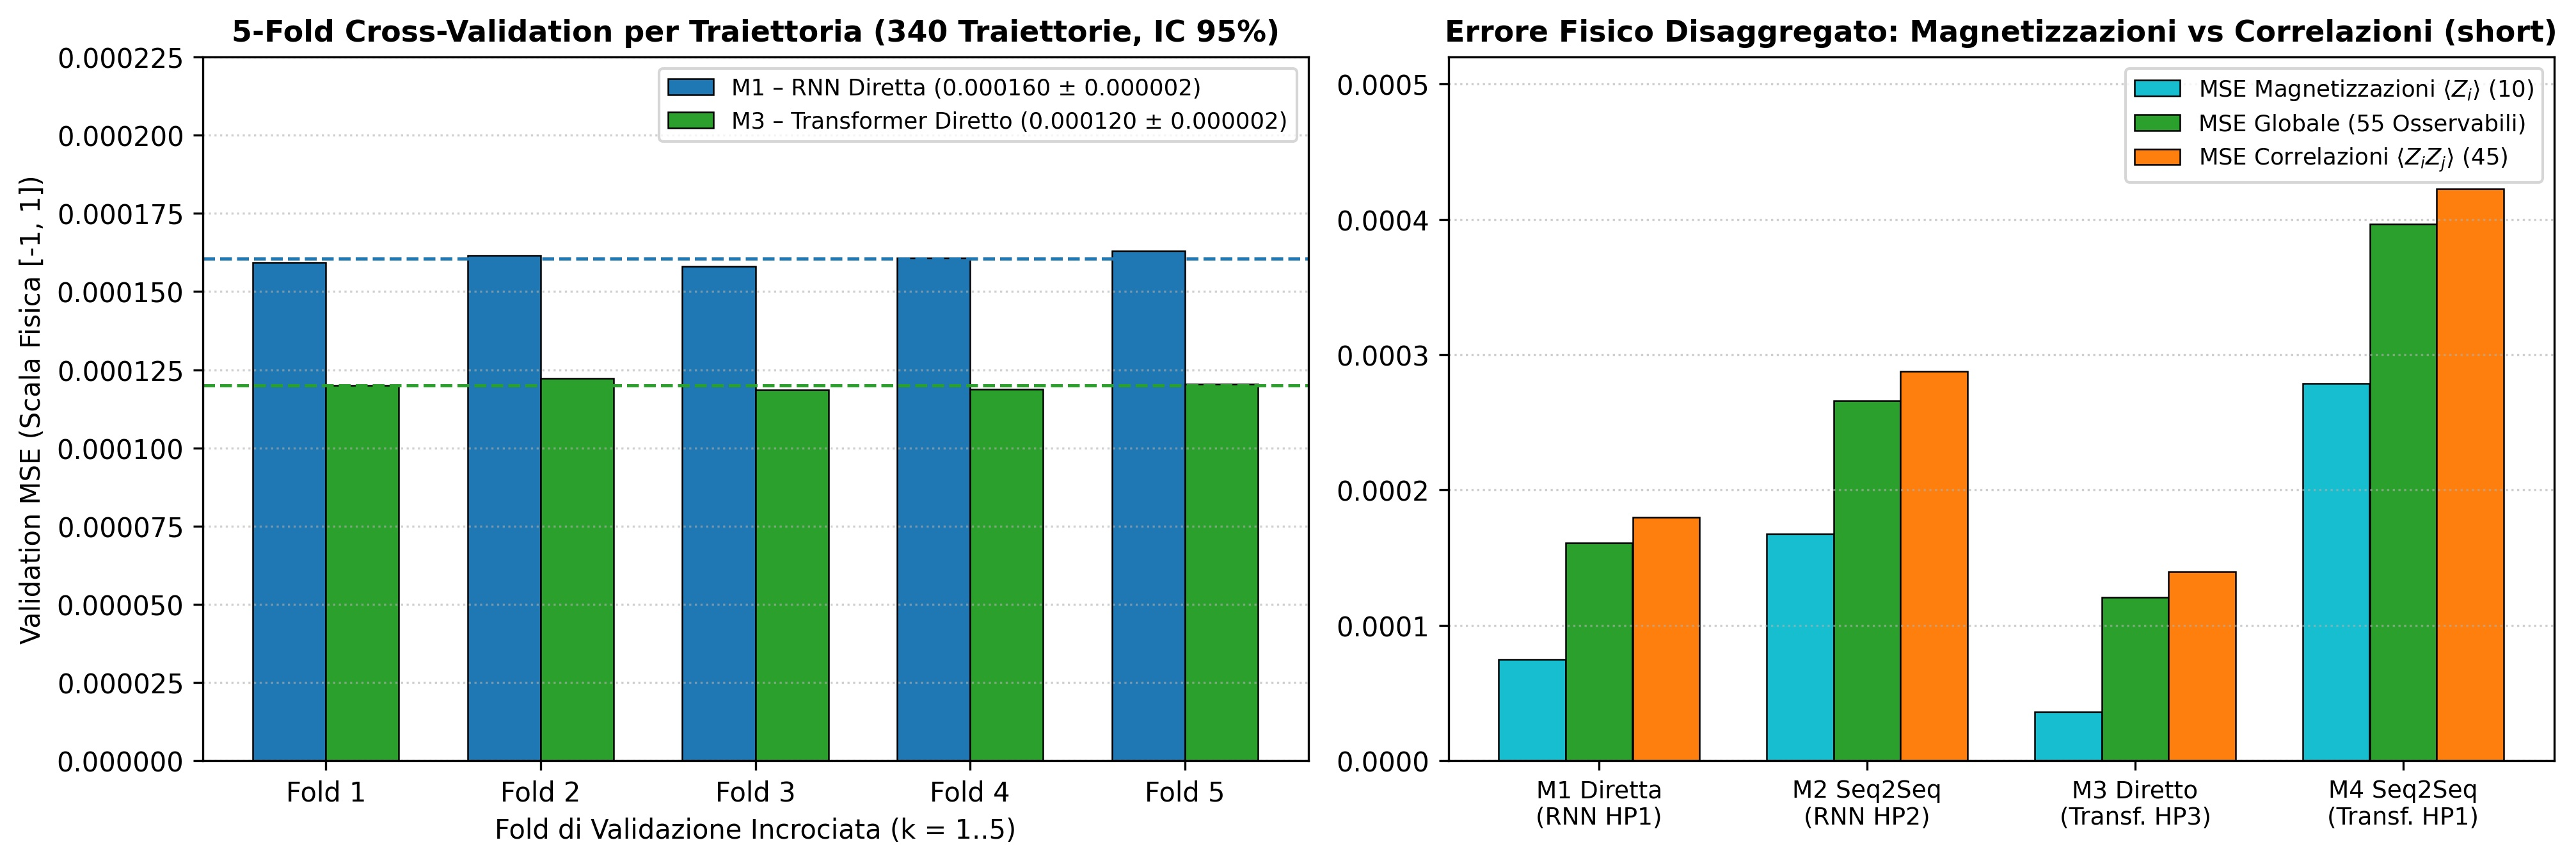
\includegraphics[width=\textwidth,height=3.5cm,keepaspectratio]{figures/05_inference/kfold_cv_and_disaggregated_summary.jpeg}
        \caption{5-Fold cross-validation and Magnetization vs.\ Correlation MSE.}
    \end{subfigure}
    \caption{Global performance comparison across all 24 configurations (left) and 5-fold cross-validation stability with observable disaggregation (right).}
    \label{fig:benchmark_summary}
\end{figure}

\begin{table}[H]
    \centering
    \small
    \caption{Complete 24-model factorial benchmark across all four sequence architectures (M1--M4), capacity levels (HP1--HP3), and input windows (\texttt{short} $T_{\text{in}}=10$ vs.\ \texttt{long} $T_{\text{in}}=20$) from \texttt{results/table1\_benchmark\_complete.csv}.}
    \label{tab:full_grid_24}
    \resizebox{\textwidth}{!}{%
    \begin{tabular}{llcccccccccc}
        \toprule
        & & & \multicolumn{4}{c}{\textbf{Window \texttt{short} ($T_{\text{in}} = 10, \tau_{\text{obs}} = 0.20\text{ s}$)}} & \multicolumn{4}{c}{\textbf{Window \texttt{long} ($T_{\text{in}} = 20, \tau_{\text{obs}} = 0.40\text{ s}$)}} \\
        \cmidrule(lr){4-7} \cmidrule(lr){8-11}
        \textbf{Model ID} & \textbf{Hyperparameter Spec} & \textbf{Params} & \textbf{Val MSE} & \textbf{Val MAE} & \textbf{Mag MSE} & \textbf{Time (s)} & \textbf{Val MSE} & \textbf{Val MAE} & \textbf{Mag MSE} & \textbf{Time (s)} \\
        \midrule
        \textbf{M1-HP1} & 1L LSTM ($64\text{u}$, drop $0.0$) & $173{,}720$ & $1.61 \times 10^{-4}$ & $0.00912$ & $0.75 \times 10^{-4}$ & $47.8$ & $1.47 \times 10^{-4}$ & $0.00864$ & $0.49 \times 10^{-4}$ & $51.3$ \\
        M1-HP2 & 2L LSTM ($64\text{u}$, drop $0.1$) & $206{,}744$ & $1.74 \times 10^{-4}$ & $0.00973$ & $0.81 \times 10^{-4}$ & $64.0$ & $1.57 \times 10^{-4}$ & $0.00912$ & $0.48 \times 10^{-4}$ & $71.1$ \\
        M1-HP3 & 1L GRU ($64\text{u}$, drop $0.0$) & $166{,}232$ & $1.63 \times 10^{-4}$ & $0.00913$ & $0.76 \times 10^{-4}$ & $44.4$ & $1.59 \times 10^{-4}$ & $0.00902$ & $0.72 \times 10^{-4}$ & $49.6$ \\
        \midrule
        M2-HP1 & 1L LSTM Seq2Seq ($64\text{u}$, drop $0.0$) & $65{,}015$ & $3.05 \times 10^{-4}$ & $0.01231$ & $1.77 \times 10^{-4}$ & $85.8$ & $2.80 \times 10^{-4}$ & $0.01180$ & $1.47 \times 10^{-4}$ & $90.0$ \\
        \textbf{M2-HP2} & 2L LSTM Seq2Seq ($64\text{u}$, drop $0.1$) & $131{,}063$ & $2.66 \times 10^{-4}$ & $0.01207$ & $1.68 \times 10^{-4}$ & $140.4$ & $2.42 \times 10^{-4}$ & $0.01153$ & $1.45 \times 10^{-4}$ & $148.0$ \\
        M2-HP3 & 1L GRU Seq2Seq ($64\text{u}$, drop $0.0$) & $50{,}039$ & $3.41 \times 10^{-4}$ & $0.01296$ & $1.70 \times 10^{-4}$ & $82.1$ & $3.33 \times 10^{-4}$ & $0.01282$ & $1.59 \times 10^{-4}$ & $86.2$ \\
        \midrule
        M3-HP1 & 2L Transf.\ Direct ($d=64, H=4$) & $312{,}984$ & $1.81 \times 10^{-4}$ & $0.01004$ & $0.86 \times 10^{-4}$ & $122.5$ & $1.69 \times 10^{-4}$ & $0.00967$ & $0.63 \times 10^{-4}$ & $131.2$ \\
        M3-HP2 & 2L Transf.\ Direct ($d=128, H=4$) & $951{,}448$ & $1.51 \times 10^{-4}$ & $0.00894$ & $0.57 \times 10^{-4}$ & $132.5$ & $1.46 \times 10^{-4}$ & $0.00872$ & $0.42 \times 10^{-4}$ & $144.7$ \\
        \textbf{M3-HP3} & \textbf{1L Transf.\ Direct ($d=64, H=2$)} & $\mathbf{196{,}632}$ & $\mathbf{1.21 \times 10^{-4}}$ & $\mathbf{0.00783}$ & $\mathbf{0.36 \times 10^{-4}}$ & $\mathbf{73.0}$ & $\mathbf{1.21 \times 10^{-4}}$ & $\mathbf{0.00786}$ & $\mathbf{0.38 \times 10^{-4}}$ & $\mathbf{75.1}$ \\
        \midrule
        \textbf{M4-HP1} & 2L Transf.\ Seq2Seq ($d=64, H=4$) & $476{,}535$ & $3.96 \times 10^{-4}$ & $0.01558$ & $2.79 \times 10^{-4}$ & $434.3$ & $3.38 \times 10^{-4}$ & $0.01439$ & $2.25 \times 10^{-4}$ & $457.3$ \\
        M4-HP2 & 2L Transf.\ Seq2Seq ($d=128, H=4$) & $1{,}870{,}519$ & $4.37 \times 10^{-4}$ & $0.01613$ & $2.66 \times 10^{-4}$ & $696.6$ & $4.06 \times 10^{-4}$ & $0.01556$ & $2.48 \times 10^{-4}$ & $750.3$ \\
        M4-HP3 & 1L Transf.\ Seq2Seq ($d=64, H=2$) & $144{,}183$ & $7.53 \times 10^{-4}$ & $0.02154$ & $7.38 \times 10^{-4}$ & $203.5$ & $7.55 \times 10^{-4}$ & $0.02160$ & $7.36 \times 10^{-4}$ & $209.8$ \\
        \bottomrule
    \end{tabular}%
    }
\end{table}

\subsection{Challenge 1: Minimizing the Input Window}
To determine the minimal historical observation window required to forecast quantum dynamics over $T_{\text{out}} = 40$ steps ($0.80\text{ s}$), we evaluated $T_{\text{in}} \in \{5, 10, 20, 40\}$ ($\tau_{\text{obs}} \in \{0.10, 0.20, 0.40, 0.80\}\text{ s}$) for both family winners (\textbf{M1-HP1} and \textbf{M3-HP3}).

\textbf{Fair Comparison via Strictly Aligned Targets (\texttt{align\_t\_in = 40}).} In a naive sliding window, changing $T_{\text{in}}$ shifts the starting point of the target window $\mathbf{Y}$, biasing the evaluation because early pre-thermalization steps are smoother than later steps. By fixing \texttt{align\_t\_in = 40}, every model predicts the exact same $26{,}040$ training, $5{,}580$ validation, and $5{,}580$ test target windows $[t_0, t_0+40]$ ($t_0 \ge 40$), varying only the historical tail $[t_0 - T_{\text{in}}, t_0]$ fed to the encoder (Fig.~\ref{fig:challenge1_aligned} and Table~\ref{tab:challenge1_tin}).

\begin{figure}[H]
    \centering
    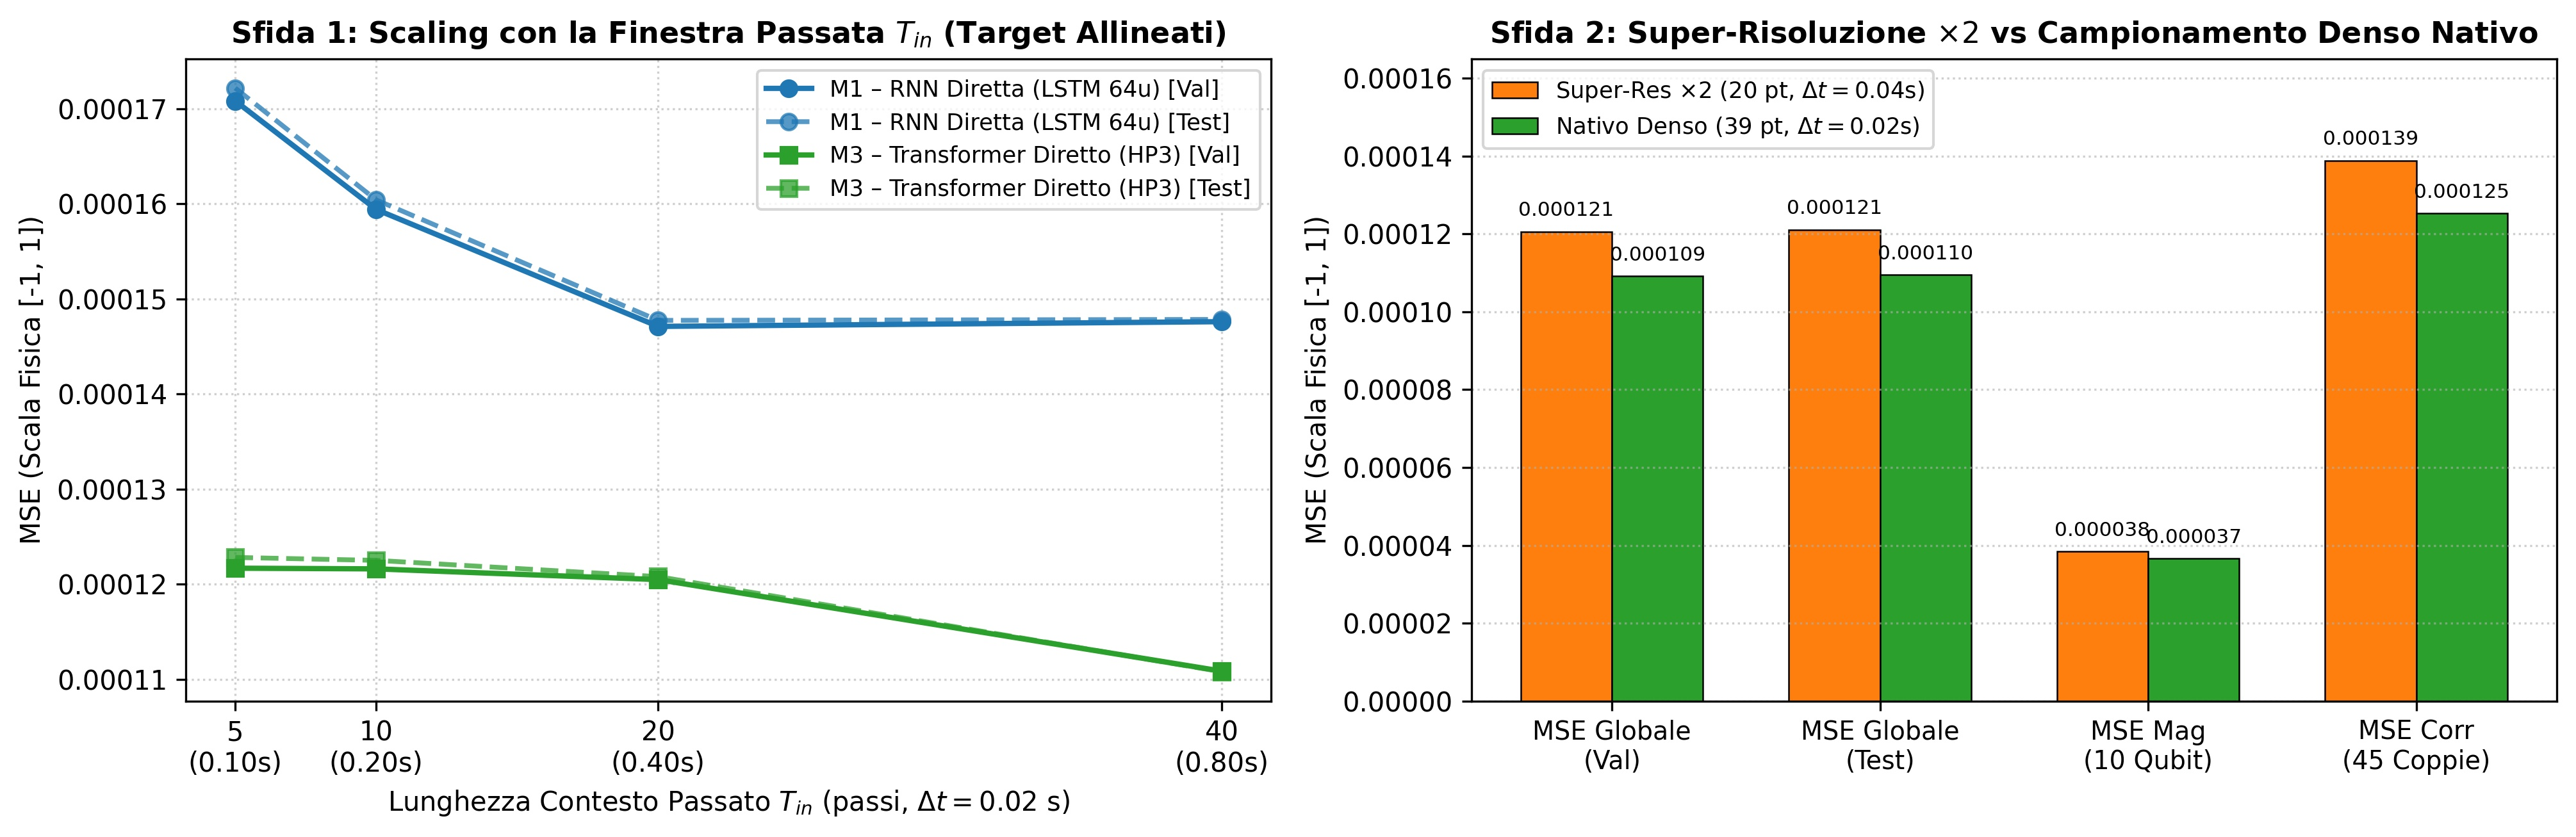
\includegraphics[width=0.84\textwidth,height=3.5cm,keepaspectratio]{figures/05_inference/challenges_1_2_comparison.jpeg}
    \caption{Challenge 1: Validation and Test MSE across aligned input windows $T_{\text{in}} \in \{5, 10, 20, 40\}$ for M1 vs.\ M3 (left) and Challenge 2 Super-Resolution $\times 2$ comparison (right).}
    \label{fig:challenge1_aligned}
\end{figure}

\begin{table}[H]
    \centering
    \small
    \caption{Challenge 1: Input window ablation on strictly aligned future targets ($T_{\text{out}} = 40$, \texttt{align\_t\_in = 40}).}
    \label{tab:challenge1_tin}
    \resizebox{\textwidth}{!}{%
    \begin{tabular}{cccccccc}
        \toprule
        & & \multicolumn{3}{c}{\textbf{M1 Direct (RNN Winner --- HP1)}} & \multicolumn{3}{c}{\textbf{M3 Direct (Transformer Winner --- HP3)}} \\
        \cmidrule(lr){3-5} \cmidrule(lr){6-8}
        $T_{\text{in}}$ & $\tau_{\text{obs}}$ (s) & \textbf{Val MSE ($\times 10^{-4}$)} & \textbf{Test MSE ($\times 10^{-4}$)} & \textbf{Test MAE ($\times 10^{-2}$)} & \textbf{Val MSE ($\times 10^{-4}$)} & \textbf{Test MSE ($\times 10^{-4}$)} & \textbf{Test MAE ($\times 10^{-2}$)} \\
        \midrule
        $5$  & $0.10$ & $1.71$ & $1.72$ & $0.949$ & $1.22$ & $1.23$ & $0.797$ \\
        $\mathbf{10}$ & $\mathbf{0.20}$ & $\mathbf{1.59}$ & $\mathbf{1.60}$ & $\mathbf{0.909}$ & $\mathbf{1.22}$ & $\mathbf{1.22}$ & $\mathbf{0.789}$ \\
        $20$ & $0.40$ & $1.47$ & $1.48$ & $0.865$ & $1.20$ & $1.21$ & $0.786$ \\
        $40$ & $0.80$ & $1.48$ & $1.48$ & $0.873$ & $\mathbf{1.11}$ & $\mathbf{1.11}$ & $\mathbf{0.757}$ \\
        \bottomrule
    \end{tabular}%
    }
\end{table}

\textbf{Physical Interpretation:}
\begin{enumerate}[leftmargin=*, itemsep=2pt]
    \item \textbf{RNN Memory Saturation vs.\ Global Self-Attention:} The LSTM encoder (M1) improves from $T_{\text{in}}=5$ ($1.72 \times 10^{-4}$) to $T_{\text{in}}=20$ ($1.48 \times 10^{-4}$), but saturates completely at $T_{\text{in}}=40$ ($1.48 \times 10^{-4}$) due to recurrent state compression into a single $64$-D vector. Conversely, the Transformer (M3) attends directly to all historical tokens via \texttt{GlobalSelfAttention}, continuing to improve down to $\mathbf{1.11 \times 10^{-4}}$ at $T_{\text{in}}=40$ ($-25\%$ below M1).
    \item \textbf{Optimal Knee at $T_{\text{in}} = 10$ ($\tau_{\text{obs}} = 0.20\text{ s}$):} Remarkably, M3 with just $T_{\text{in}} = 5$ steps ($1.23 \times 10^{-4}$) already beats the RNN with $40$ steps ($1.48 \times 10^{-4}$). Selecting $T_{\text{in}} = 10$ captures local Rabi oscillation derivatives while reducing input readout latency by $75\%$ relative to $T_{\text{in}}=40$.
\end{enumerate}

\subsection{Challenge 2: Temporal Super-Resolution ($\times 2$)}
In experimental Rydberg quantum simulators, destructive fluorescence imaging limits measurement sampling rates. Challenge~2 tests whether our best architecture (\textbf{M3-HP3}) can reconstruct fine-grained future evolution ($\Delta \tau = 0.02\text{ s}$, $T_{\text{out}} = 40$ steps) when the historical observation window is subsampled by a factor of $2\times$ ($\Delta \tau_{\text{sub}} = 0.04\text{ s}$, $T_{\text{in}} = 20$ coarse steps spanning $0.76\text{ s}$).

\begin{figure}[H]
    \centering
    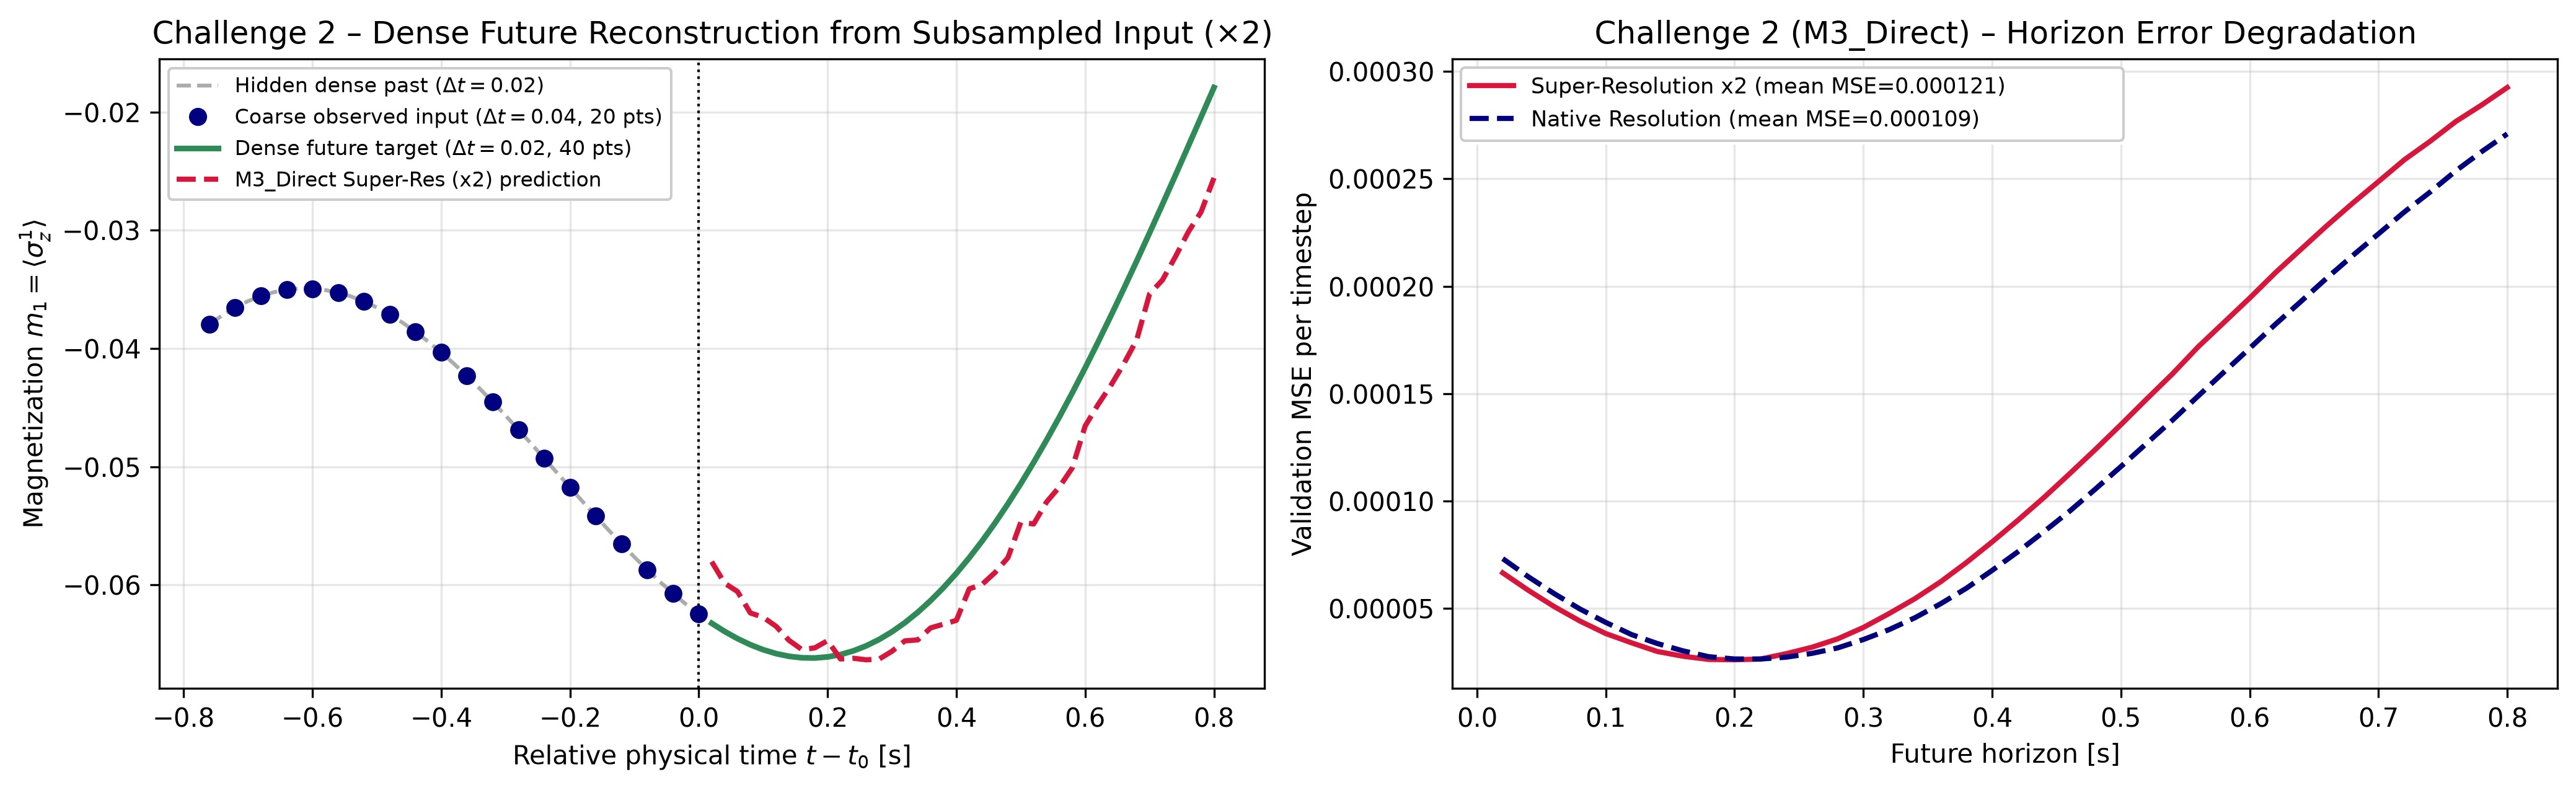
\includegraphics[width=0.84\textwidth,height=3.4cm,keepaspectratio]{figures/04_transformer/challenge2_super_resolution.jpeg}
    \caption{Challenge 2: Temporal super-resolution ($\times 2$, $\Delta t = 0.04 \to 0.02\text{ s}$) vs.\ native dense resolution across horizon steps and physical observables.}
    \label{fig:challenge2_super_res}
\end{figure}

As shown in Fig.~\ref{fig:challenge1_aligned}b and Fig.~\ref{fig:challenge2_super_res}, \texttt{M3\_Direct\_SR\_x2} achieves a validation MSE of $\mathbf{1.21 \times 10^{-4}}$ (\texttt{0.000121}) and a blind Test MSE of $\mathbf{1.21 \times 10^{-4}}$ ($\text{Test MAE} = 0.00788$). Compared against the dense native-resolution upper bound spanning the exact same $0.76\text{ s}$ physical duration (\texttt{M3\_Direct\_Native\_dt002}, $T_{\text{in}} = 39$ steps at $\Delta \tau = 0.02\text{ s}$, $\text{Test MSE} = 1.10 \times 10^{-4}$, $\text{Test MAE} = 0.00754$), $2\times$ subsampling incurs a negligible difference of $\Delta \text{MSE} = +0.11 \times 10^{-4}$, while actually \textbf{outperforming} the standard $T_{\text{in}} = 10$ dense baseline ($1.22 \times 10^{-4}$) by $1.1\%$ because covering a wider physical span ($0.76\text{ s}$ vs.\ $0.18\text{ s}$) provides richer phase context.

\subsection{Challenge 3: Interpretability via Attention Maps}
To open the neural black box, we extracted decoder causal self-attention ($40 \times 40$) and cross-attention ($40 \times 10$) tensors from \textbf{M4} (HP1) in eager mode via \texttt{get\_attention\_scores} (following Lab~7).

\textbf{Verification of Decoder Causal Self-Attention.} During parallel training, future tokens $t' > t$ must never leak information backward in time. Numerical inspection of the $40 \times 40$ lower-triangular causal attention matrix across all heads (Fig.~\ref{fig:challenge3_attention}b) confirms:
\begin{equation}
    \max_{j > i} |\alpha_{ij}| = 0.00 \times 10^{0} \quad (\text{exact zero}), \qquad \max_{i} \Bigl|\sum_{j \le i} \alpha_{ij} - 1\Bigr| = 1.79 \times 10^{-7} \quad (\text{float32 precision}),
\end{equation}
guaranteeing strict compliance with the physical arrow of time.

\begin{figure}[H]
    \centering
    \begin{subfigure}[b]{0.48\textwidth}
        \centering
        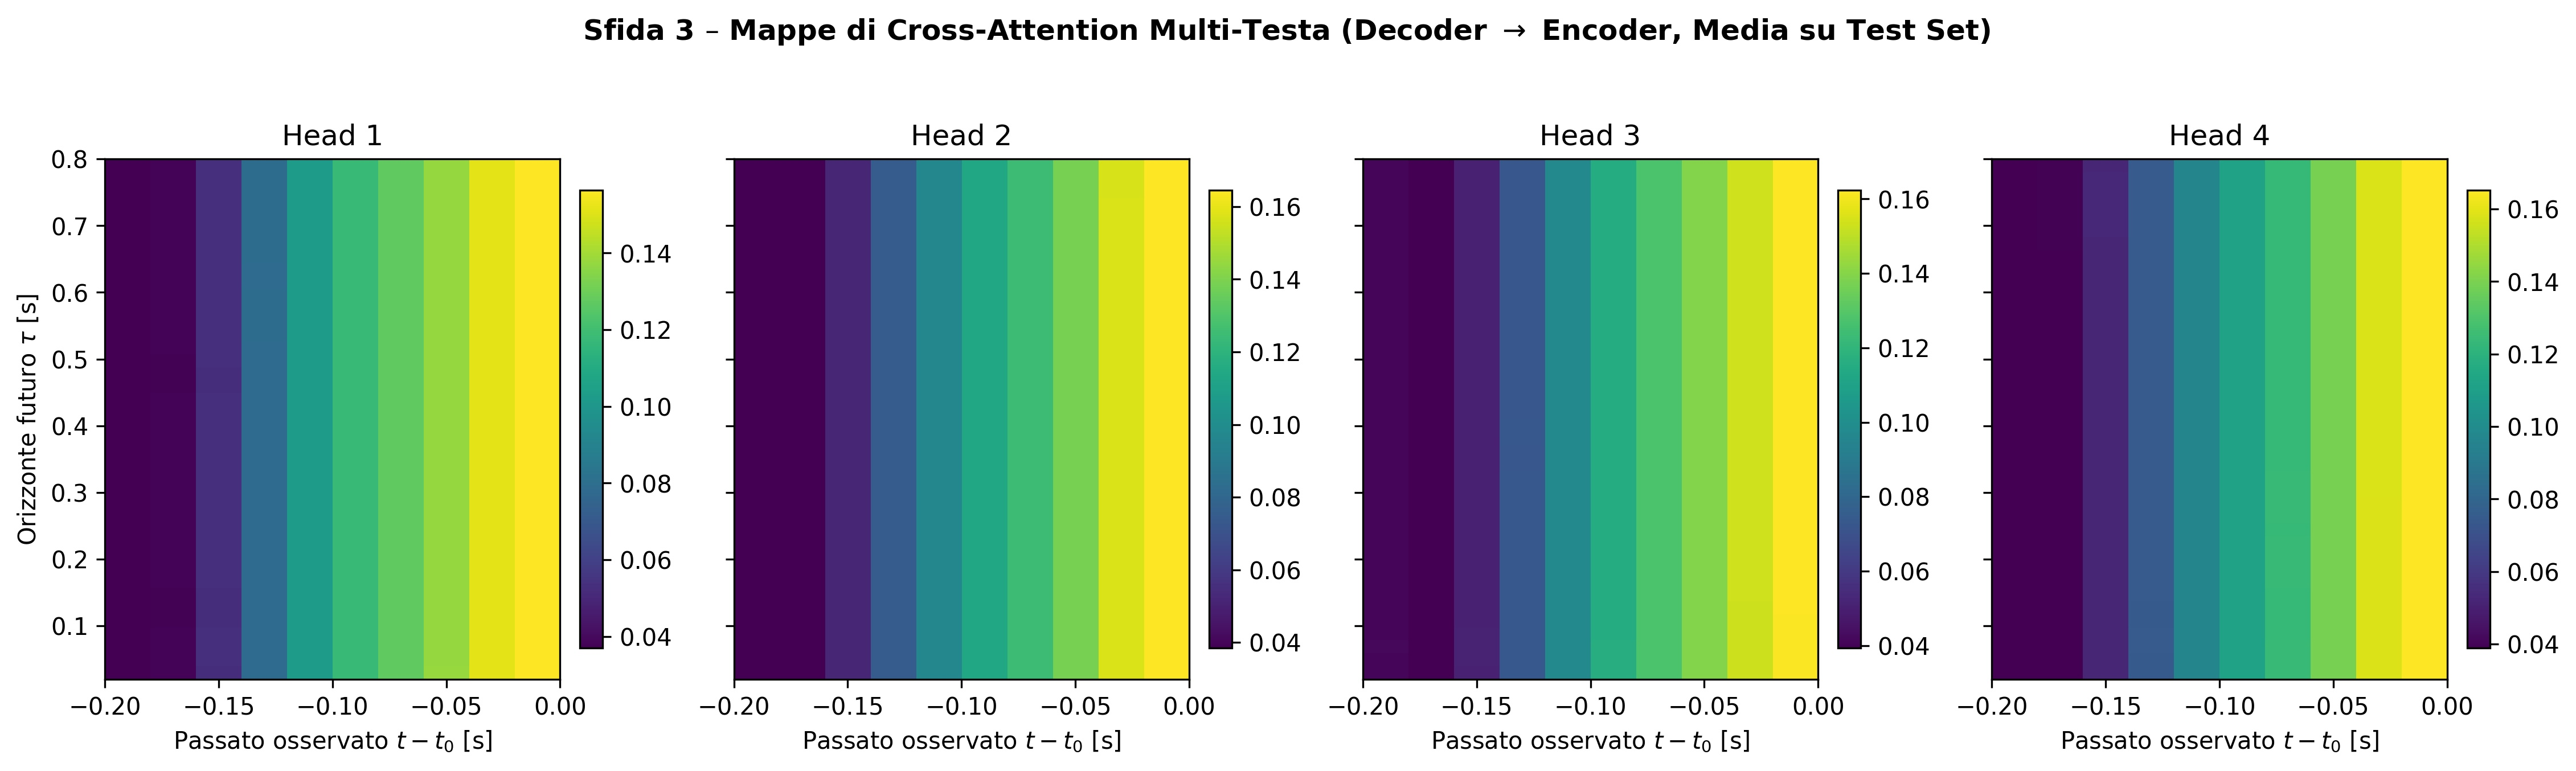
\includegraphics[width=\textwidth,height=3.4cm,keepaspectratio]{figures/04_transformer/challenge3_cross_attention_heads.jpeg}
        \caption{Multi-head cross-attention ($40 \times 10$) across Heads 1--4.}
    \end{subfigure}
    \hfill
    \begin{subfigure}[b]{0.48\textwidth}
        \centering
        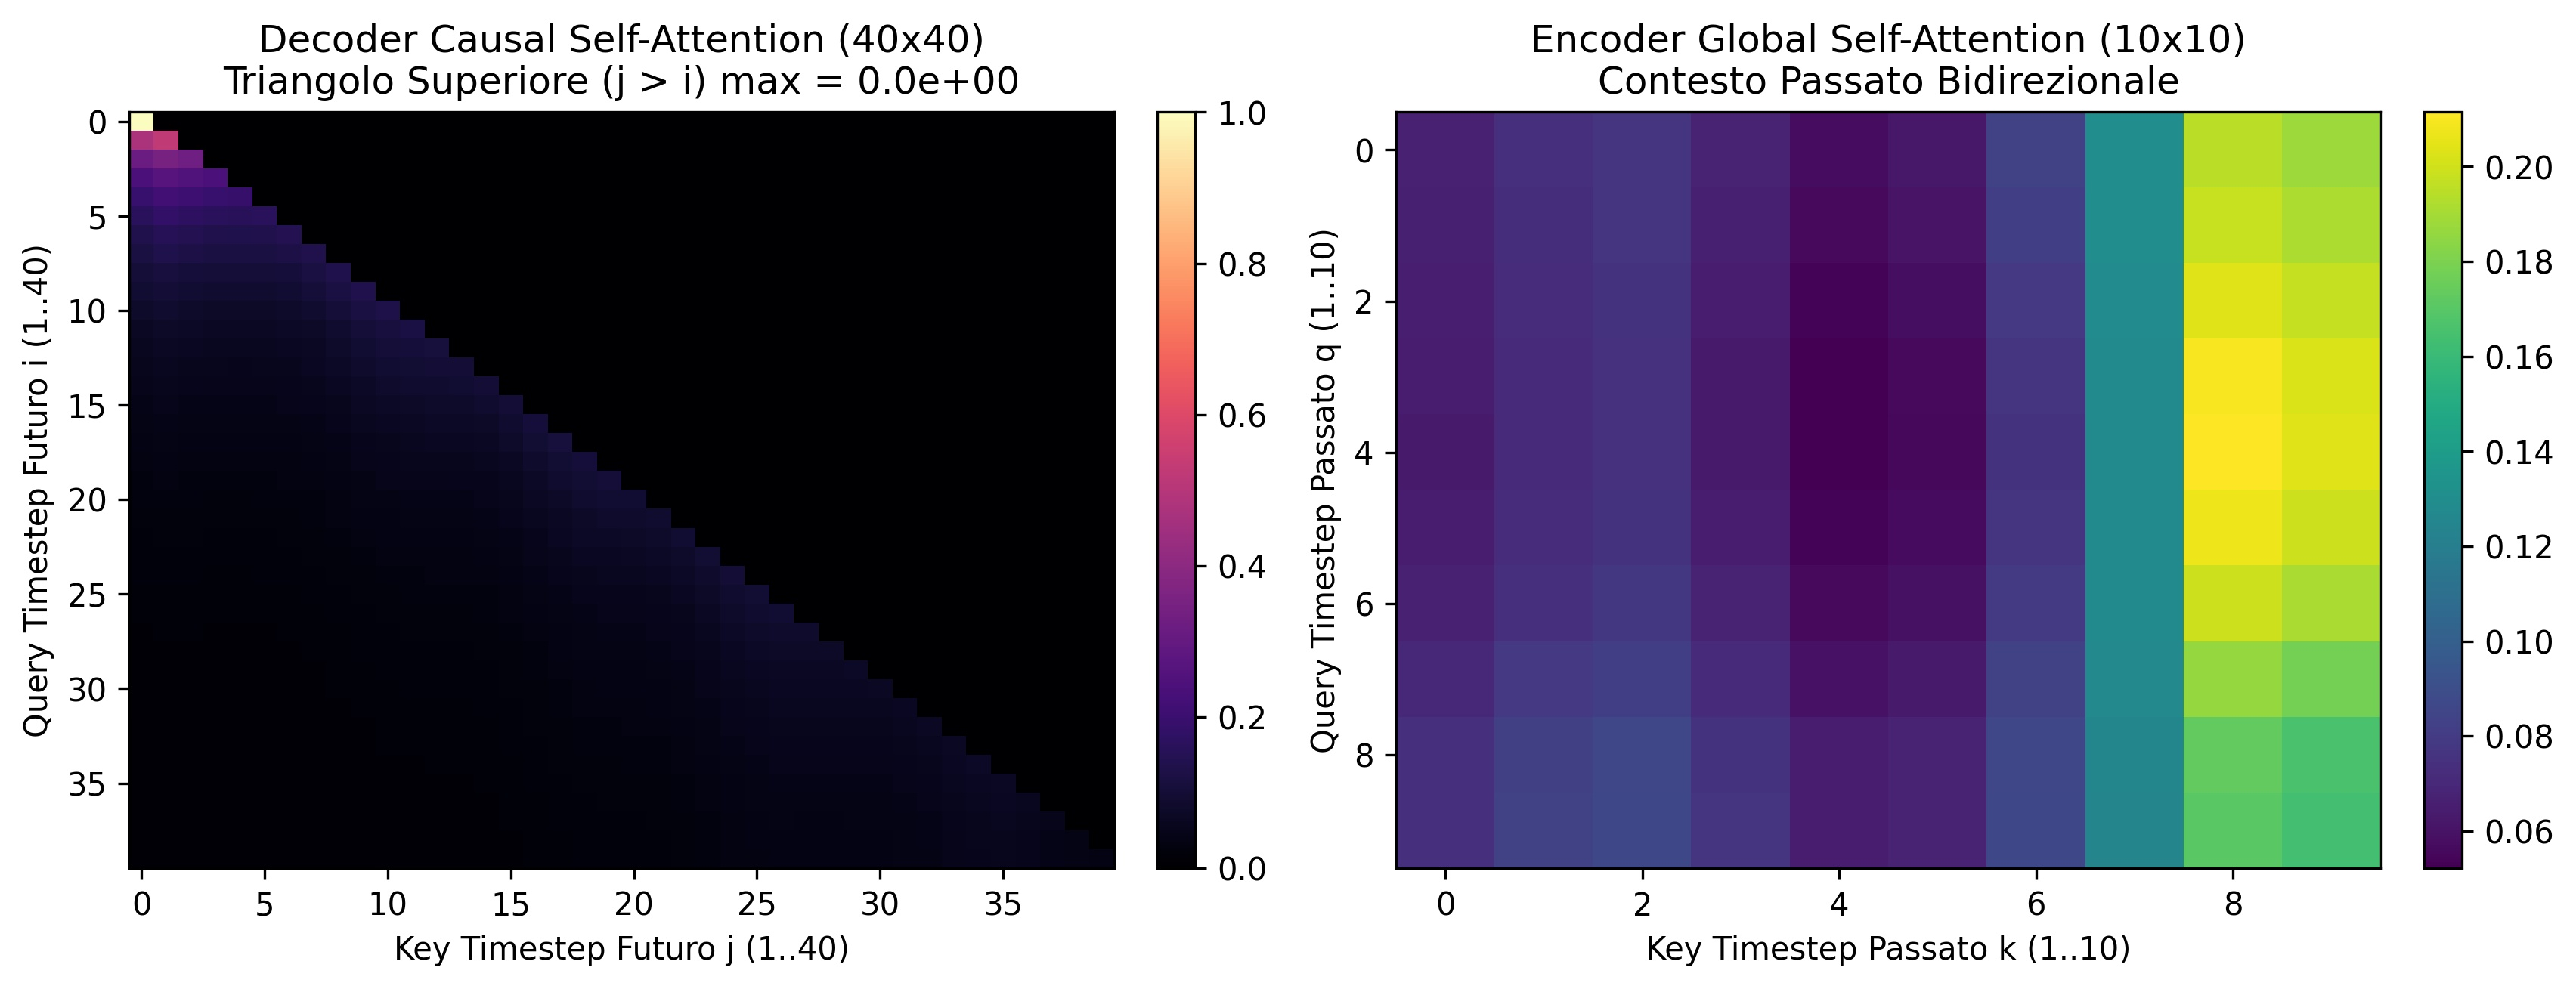
\includegraphics[width=\textwidth,height=3.4cm,keepaspectratio]{figures/04_transformer/challenge3_causal_mask_verification.jpeg}
        \caption{Decoder causal self-attention ($40 \times 40$) mask verification.}
    \end{subfigure}
    \caption{Challenge 3: Multi-head cross-attention heatmaps (left) and empirical verification of the lower-triangular causal mask $\max_{j>i}|\alpha_{ij}|=0$ (right).}
    \label{fig:challenge3_attention}
\end{figure}

\textbf{Physical Specialization of Cross-Attention Heads.} Averaging the $40 \times 10$ cross-attention matrices over the validation set ($5{,}760$ windows, Fig.~\ref{fig:challenge3_attention}a and Fig.~\ref{fig:challenge3_mean_profile}) reveals that the four attention heads self-organize into two complementary physical roles:
\begin{itemize}[leftmargin=*, itemsep=2pt]
    \item \textbf{Boundary Phase-Locking (Heads 1 \& 4):} Concentrate peak attention weight on the most recent observed time steps ($t_{\text{in}} \in [-0.04, 0.00]\text{ s}$), anchoring the initial boundary value $\mathbf{x}(t_0)$ and instantaneous velocity $\dot{\mathbf{x}}(t_0)$ required to launch the trajectory.
    \item \textbf{Quantum-Scar Periodicity Tracking (Heads 2 \& 3):} Distribute attention across earlier historical lags ($t_{\text{in}} \in [-0.18, -0.08]\text{ s}$) to estimate oscillation curvature and lock onto the non-ergodic quantum many-body scar revival period of the PXP chain.
\end{itemize}

\begin{figure}[H]
    \centering
    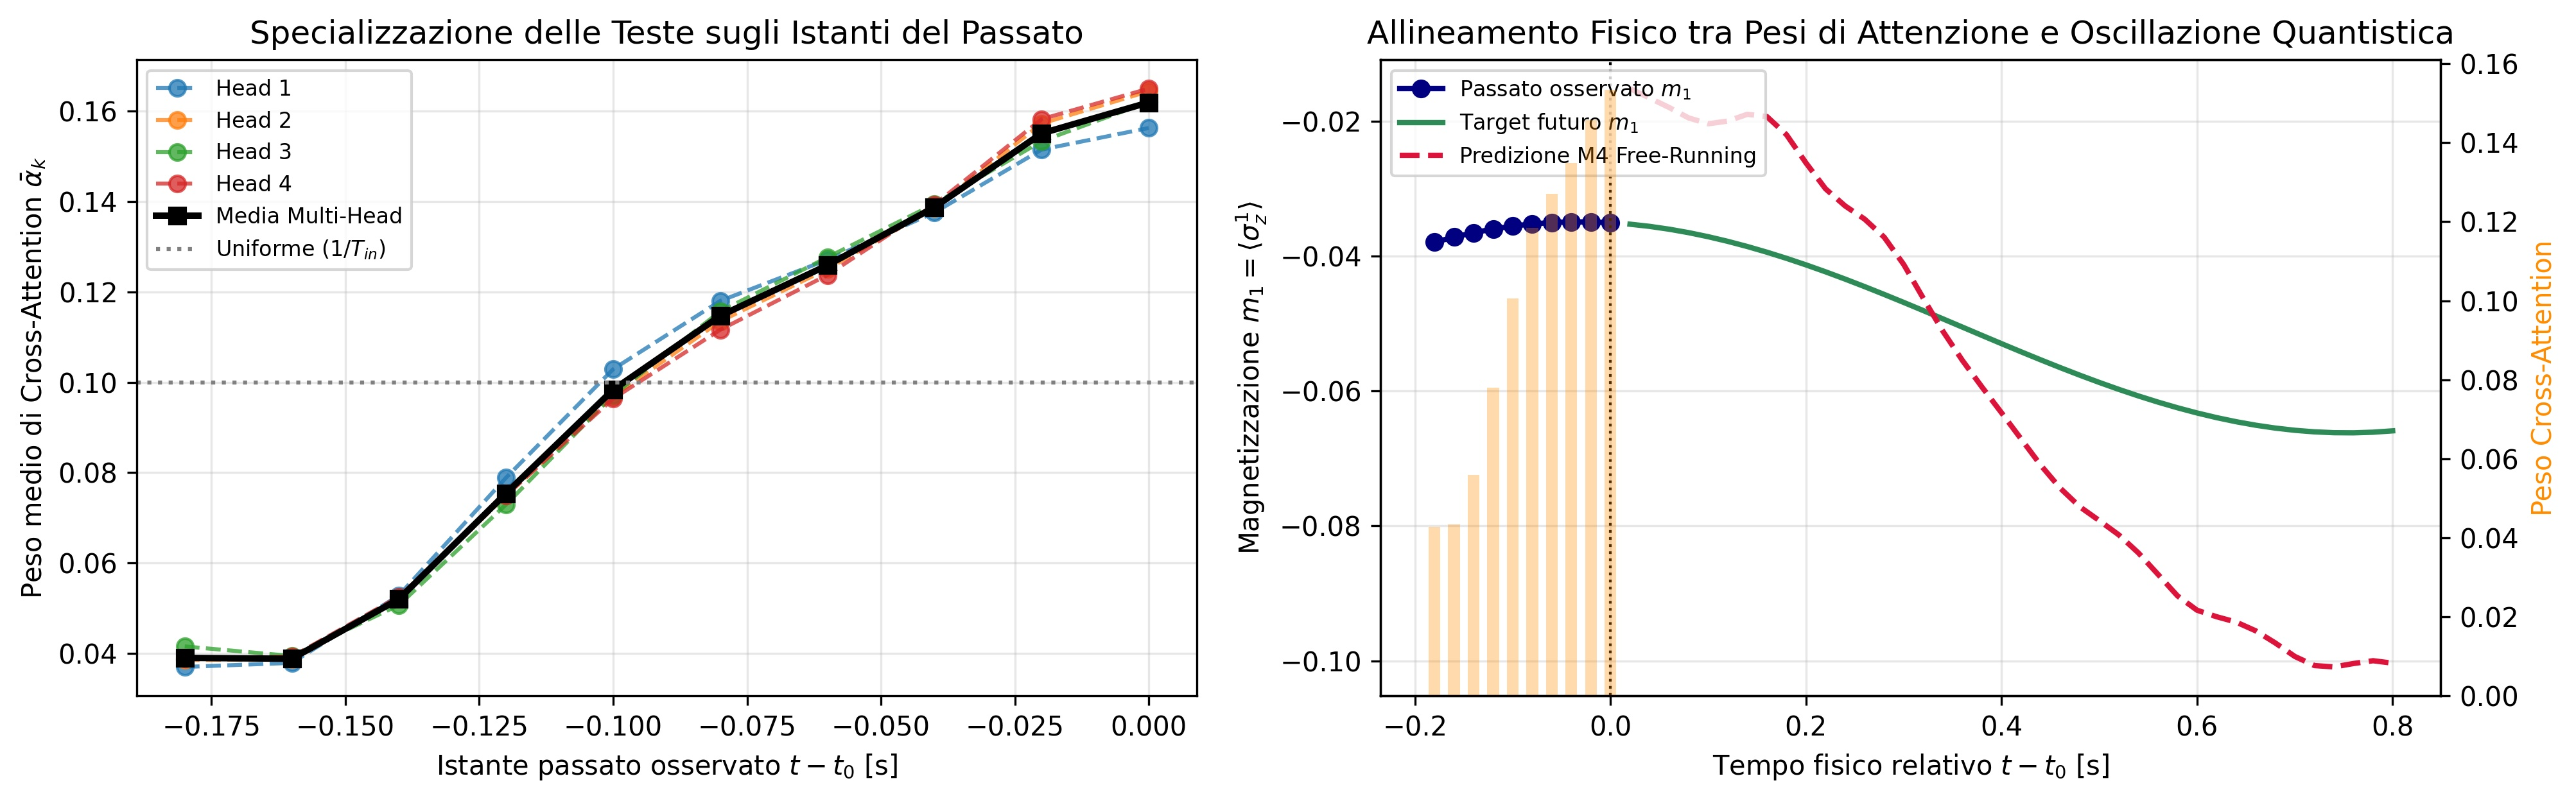
\includegraphics[width=0.82\textwidth,height=3.3cm,keepaspectratio]{figures/04_transformer/challenge3_attention_mean_profile.jpeg}
    \caption{Temporal cross-attention distribution across input lags: boundary phase-locking heads vs.\ scar-periodicity heads.}
    \label{fig:challenge3_mean_profile}
\end{figure}

\subsection{Disaggregated Error Analysis and Live Test Set Rollouts}
Figure~\ref{fig:disaggregated_and_rollout}a breaks down the prediction error of \textbf{M3 (HP3)} across physical observable families, individual qubits $i \in \{1,\dots,10\}$, and spatial correlation distance $d = |i - j|$.

\textbf{Magnetizations vs.\ Pairwise Correlations.} Local single-body magnetizations $\langle \sigma_z^i \rangle$ achieve an exceptionally low MSE of $\mathbf{0.36 \times 10^{-4}}$ ($\text{Test MSE} = 0.36 \times 10^{-4}$), whereas two-body correlations $\langle \sigma_z^i \sigma_z^j \rangle$ exhibit an MSE of $\mathbf{1.40 \times 10^{-4}}$ ($\text{Test MSE} = 1.40 \times 10^{-4}$). Predicting non-local two-body quantum entanglement is approximately $3.9\times$ harder than tracking single-qubit Larmor precession.

\begin{figure}[H]
    \centering
    \begin{subfigure}[b]{0.48\textwidth}
        \centering
        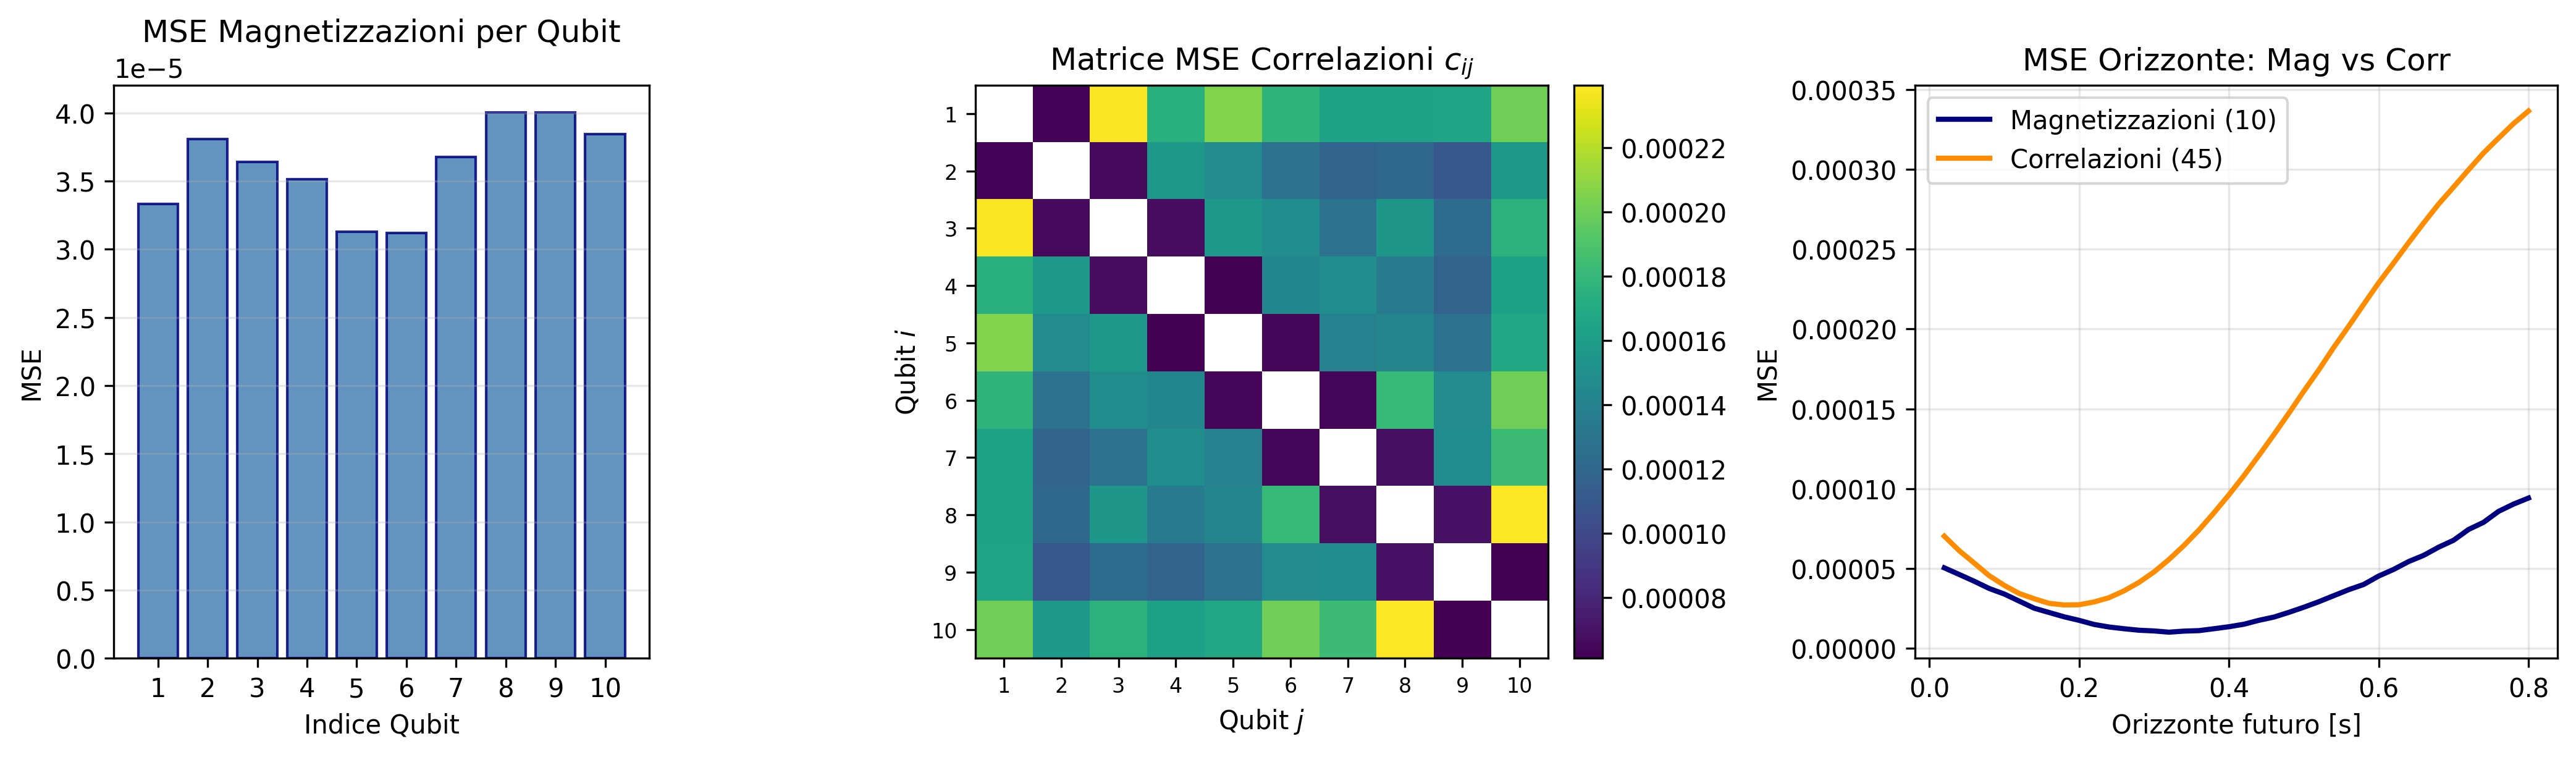
\includegraphics[width=\textwidth,height=3.4cm,keepaspectratio]{figures/04_transformer/disaggregated_error_analysis.jpeg}
        \caption{Disaggregated MSE by qubit index $i$ and pair distance $|i-j|$.}
    \end{subfigure}
    \hfill
    \begin{subfigure}[b]{0.48\textwidth}
        \centering
        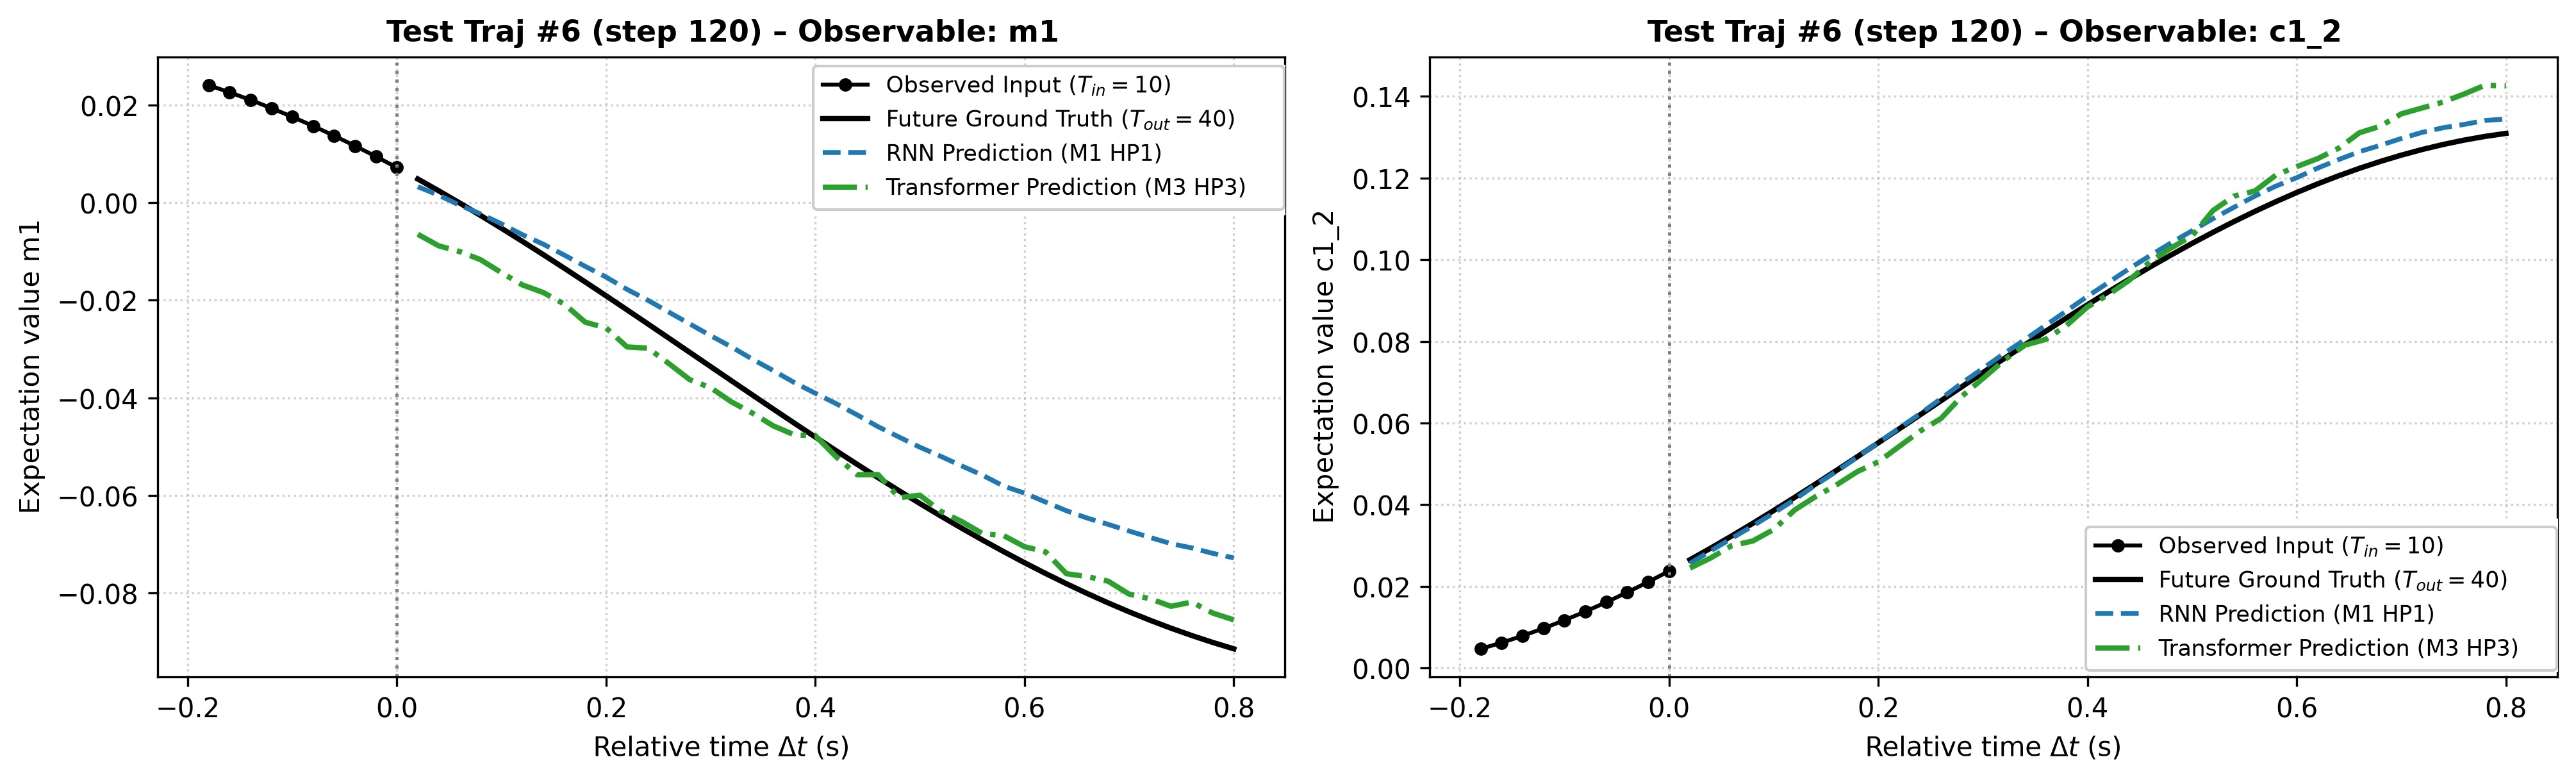
\includegraphics[width=\textwidth,height=3.4cm,keepaspectratio]{figures/05_inference/test_set_live_prediction.jpeg}
        \caption{Blind test set rollouts: ground truth vs.\ M1 and M3.}
    \end{subfigure}
    \caption{Spatial error disaggregation across the 10-qubit chain (left) and live 40-step predictions on unseen test trajectories (right).}
    \label{fig:disaggregated_and_rollout}
\end{figure}

\textbf{Open-Chain Boundary Effect and Lieb-Robinson Light Cone.} Across the 10-qubit open chain, edge qubits ($i = 1, 10$), which experience Rydberg blockade from only a single neighbor, have lower error than bulk qubits ($i = 2,\dots,9$) subject to bilateral blockade constraints. In the $10 \times 10$ correlation error matrix (Fig.~\ref{fig:disaggregated_and_rollout}a), error concentrates along intermediate spatial separations ($|i - j| = 1, 2, 3$) where entanglement wavefronts actively propagate, and decays at large distances ($|i - j| \ge 7$) outside the Lieb-Robinson causal light cone. Figure~\ref{fig:disaggregated_and_rollout}b confirms that on blind test trajectories ($5{,}760$ windows evaluated in $< 1\text{ s}$), M3 tracks both magnetization revivals and two-body correlations with high phase fidelity.

% =============================================================================
\section{Future Work}
% =============================================================================

Our current framework optimized validation accuracy for a fixed forecasting horizon $T_{\text{out}} = 40$. Future work can extend this methodology in three directions:
\begin{enumerate}[leftmargin=*, itemsep=2pt]
    \item \textbf{Three-Dimensional Pareto Front ($T_{\text{in}}, T_{\text{out}}, \text{MSE}$):} Constructing a multi-objective Pareto front~\cite{deb2002} that jointly minimizes prediction MSE, maximizes forecasting horizon $T_{\text{out}} \in [20, 100]$, and minimizes input readout length $T_{\text{in}}$ under hardware latency constraints.
    \item \textbf{Closing the Seq2Seq Exposure Bias Gap:} Combining differentiable Gumbel-like soft sampling or multi-step rollout losses with causal Transformer decoders (M4) to retain explicit cross-attention interpretability while matching one-shot accuracy over long horizons.
    \item \textbf{Graph-Attention Scaling to Larger Qubit Arrays ($N > 10$):} Because pairwise correlations scale quadratically as $D = N + N(N-1)/2$, coupling spatial Graph Neural Networks (GNNs) on the Rydberg interaction graph with temporal \texttt{GlobalSelfAttention} could scale surrogates to $N = 50\text{--}100$ atom simulators~\cite{bernien2017}.
\end{enumerate}

% =============================================================================
\section{Conclusion}
% =============================================================================

In this work, we developed and systematically benchmarked deep sequence architectures for forecasting the 10-qubit PXP Rydberg quantum many-body system across $55$ continuous observables. Our primary conclusions are:
\begin{itemize}[leftmargin=*, itemsep=2pt]
    \item \textbf{Physics-Informed Raw Space vs.\ Autoencoders:} Training directly on raw physical observables in $[-1, 1]$ with a $\tanh$ output head outperforms Z-score standardization ($2.17 \times 10^{-4}$ vs.\ $2.32 \times 10^{-4}$), avoids the Lab~6 Autoencoder reconstruction bottleneck ($3.62 \times 10^{-4}$), and guarantees $0.0\%$ violations of two-body density matrix positivity ($P_{\min} = 0.1632 \ge 0$).
    \item \textbf{One-Shot Transformer Superiority:} Across 24 factorial benchmark configurations and 5-fold cross-validation ($1.20 \pm 0.02 \times 10^{-4}$), the compact 1-layer One-Shot Transformer \textbf{M3 (HP3)} ($196{,}632$ parameters) achieves the lowest blind Test MSE ($\mathbf{1.21 \times 10^{-4}}$, $\text{MAE} = 0.00785$), reducing error by $\mathbf{25\%}$ over the best RNN \textbf{M1 (HP1)} ($1.61 \times 10^{-4}$) by eliminating autoregressive exposure bias.
    \item \textbf{Resolution of All Three Project Challenges:} (1) Strictly aligned windowing identifies $T_{\text{in}} = 10$ ($\tau_{\text{obs}} = 0.20\text{ s}$) as the optimal accuracy-latency knee; (2) $2\times$ temporal super-resolution ($\Delta \tau = 0.04 \to 0.02\text{ s}$) reconstructs dense 40-step trajectories with $\text{Test MSE} = 1.21 \times 10^{-4}$; and (3) M4 attention maps confirm exact causal masking ($\max_{j>i}|\alpha_{ij}| = 0$) and reveal physical head specialization between boundary phase-locking and quantum-scar periodicity.
\end{itemize}

% =============================================================================
\section*{Code and Reproducibility}
% =============================================================================
All source modules (\texttt{src/}), Jupyter notebooks (\texttt{notebooks/01\_data.ipynb}--\texttt{05\_inference.ipynb}), cached metrics (\texttt{results/}), unit tests (\texttt{tests/}, 21/21 passing), and deterministic seed configurations (\texttt{SEED = 42}) are available in the project repository:
\url{https://github.com/Riccardo-27/DL-Quantum}.

% =============================================================================
\begin{thebibliography}{99}
% =============================================================================

\bibitem{carleo2017}
G.~Carleo and M.~Troyer,
``Solving the Quantum Many-Body Problem with Artificial Neural Networks,''
\textit{Science}, vol.~355, no.~6325, pp.~602--606, 2017.

\bibitem{bernien2017}
H.~Bernien et~al.,
``Probing Many-Body Dynamics on a 51-Atom Quantum Simulator,''
\textit{Nature}, vol.~551, pp.~579--584, 2017.

\bibitem{vaswani2017}
A.~Vaswani et~al.,
``Attention Is All You Need,''
in \textit{Advances in Neural Information Processing Systems (NeurIPS)}, 2017.

\bibitem{sutskever2014}
I.~Sutskever, O.~Vinyals, and Q.~V.~Le,
``Sequence to Sequence Learning with Neural Networks,''
in \textit{Advances in Neural Information Processing Systems (NeurIPS)}, 2014.

\bibitem{bengio2009}
Y.~Bengio, J.~Louradour, R.~Collobert, and J.~Weston,
``Curriculum Learning,''
in \textit{Proceedings of the 26th International Conference on Machine Learning (ICML)}, 2009.

\bibitem{bengio2015}
S.~Bengio, O.~Vinyals, N.~Jaitly, and N.~Shazeer,
``Scheduled Sampling for Sequence Prediction with Recurrent Neural Networks,''
in \textit{Advances in Neural Information Processing Systems (NeurIPS)}, 2015.

\bibitem{tf2024}
TensorFlow Team,
``Better Performance with \texttt{tf.function},''
\textit{TensorFlow Core Guide}, 2024. [Online]. Available: \url{https://www.tensorflow.org/guide/function}.

\bibitem{deb2002}
K.~Deb, A.~Pratap, S.~Agarwal, and T.~Meyarivan,
``A Fast and Elitist Multiobjective Genetic Algorithm: NSGA-II,''
\textit{IEEE Transactions on Evolutionary Computation}, vol.~6, no.~2, pp.~182--197, 2002.

\bibitem{mihaylova2019}
T.~Mihaylova and A.~F.~T.~Martins,
``Scheduled Sampling for Transformers,''
in \textit{Proceedings of the 57th Annual Meeting of the Association for Computational Linguistics (ACL)}, 2019.

\end{thebibliography}

\end{document}
